% ============================================================
% A4 Landscape Exam Cheat Sheet Template
% 4 columns per page, 2 pages (i.e. 8 columns total)
% ============================================================
\documentclass[10pt]{extarticle}

% ---------- Page geometry: A4 landscape, tight margins ----------
\usepackage[a4paper, landscape, margin=0.4cm]{geometry}

\usepackage{tikz}
\usetikzlibrary{arrows.meta, positioning, shapes.geometric}

\usepackage{amsmath}
\usepackage{array}
\usepackage{multirow}
\usepackage{bigdelim}

\usepackage{graphicx}
\usepackage{mathtools}
\usepackage{subcaption}

% ---------- Multi-column layout ----------
\usepackage{multicol}
\setlength{\columnsep}{0.5cm}
\setlength{\columnseprule}{0.4pt}

% ---------- Fonts & sizing ----------
\usepackage[utf8]{inputenc}
\usepackage[T1]{fontenc}
\renewcommand{\familydefault}{\sfdefault}

% ---------- Math ----------
\usepackage{amsmath, amssymb, amsthm}

% ---------- Compact spacing ----------
\usepackage{titlesec}
\usepackage{enumitem}
\setlist{nosep, leftmargin=1.1em, itemsep=0pt, parsep=0pt, topsep=1pt}

% Compact section headers
\titleformat{\section}
{\normalfont\bfseries\small\color{black}}
{}{0em}{}
\titlespacing{\section}{0pt}{4pt}{2pt}

\titleformat{\subsection}
{\normalfont\bfseries\footnotesize}
{}{0em}{}
\titlespacing{\subsection}{0pt}{3pt}{1pt}

% ---------- Misc useful packages ----------
\usepackage{graphicx}
\usepackage{array}
\usepackage{booktabs}
\usepackage{xcolor}
\usepackage{tcolorbox}
\tcbuselibrary{skins, breakable}

% Remove page numbers / headers footers to save space
\usepackage{fancyhdr}
\pagestyle{empty}

% Zero out paragraph indent/skip to save vertical space
\setlength{\parindent}{0pt}
\setlength{\parskip}{0pt}

% Tiny custom box for formulas / key results
\newtcolorbox{formulabox}[1][]{
  colback=gray!5, colframe=black!60,
  boxrule=0.3pt, arc=1pt,
  left=2pt, right=2pt, top=1pt, bottom=1pt,
  #1
}

% Shortcut for a compact rule under section titles
\newcommand{\sectionrule}{\vspace{-2pt}\hrule\vspace{2pt}}

% Draw UDP diagram
\newcommand{\udpdiagram}{%
  \begin{center}
    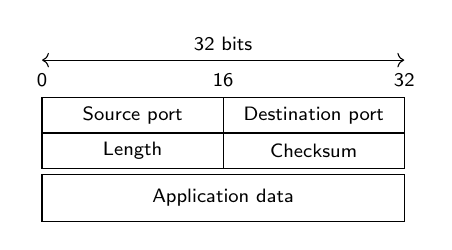
\begin{tikzpicture}[
        font=\scriptsize,
        cell/.style={
          draw,
          minimum height=0.45cm,
          minimum width=2.3cm,
          align=center,
          inner sep=2pt
        }
      ]

      \node at (0,1.25) {0};
      \node at (2.3,1.25) {16};
      \node at (4.6,1.25) {32};

      \draw[<->] (0,1.50) -- node[above] {32 bits} (4.6,1.50);

      \node[cell] at (1.15,0.8) {Source port};
      \node[cell] at (3.45,0.8) {Destination port};

      \node[cell] at (1.15,0.35) {Length};
      \node[cell] at (3.45,0.35) {Checksum};

      \node[
        draw,
        minimum width=4.6cm,
        minimum height=0.6cm,
        align=center,
        inner sep=2pt
      ] at (2.3,-0.25) {Application data};

    \end{tikzpicture}
  \end{center}%
}

% Embedded Go-Back-N loss/recovery timeline, matching the lecture diagram.
\definecolor{gbnblue}{RGB}{0,0,170}
\definecolor{gbngreen}{RGB}{45,135,35}
\definecolor{gbnred}{RGB}{220,55,45}
\definecolor{gbncyan}{RGB}{65,190,235}
\newcommand{\gbnwindowrow}[2]{%
  \foreach \i in {0,...,7}{%
    \pgfmathtruncatemacro{\gbnselected}{(\i>=#2)*(\i<#2+4)}%
    \ifnum\gbnselected=1
    \fill[gbnblue] ({.02+.36*\i},#1-.25) rectangle ({.37+.36*\i},#1+.25);
    \node[text=white,font=\tiny] at ({.195+.36*\i},#1) {\i};
    \else
    \node[font=\tiny] at ({.195+.36*\i},#1) {\i};
    \fi
  }%
}
\newcommand{\gobackndiagram}{%
  \resizebox{.98\linewidth}{!}{%
    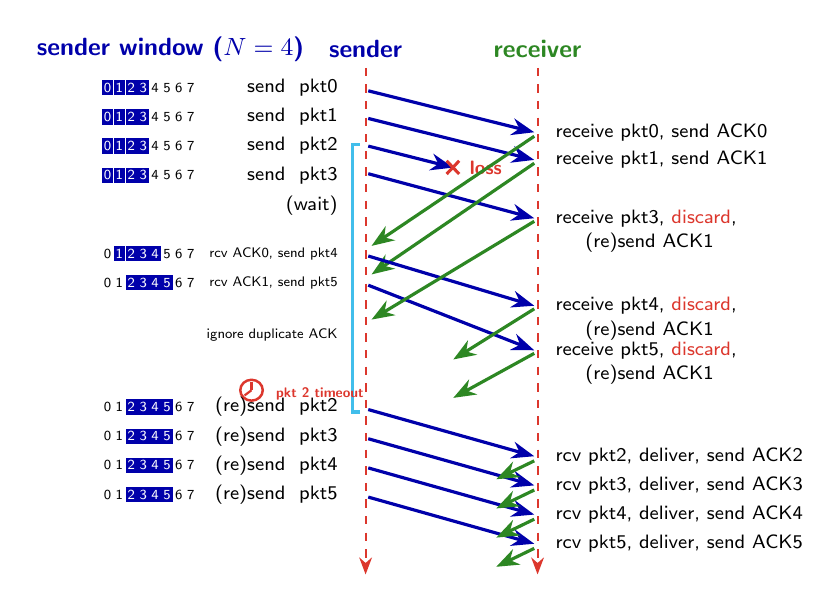
\begin{tikzpicture}[x=.42cm,y=.39cm,>=Stealth,
        data/.style={->,draw=gbnblue,line width=1.15pt},
        ack/.style={->,draw=gbngreen,line width=1.15pt},
      life/.style={gbnred,dashed,line width=.7pt}]
      % Headers and the sender-window snapshots.
      \node[gbnblue,font=\bfseries\itshape\small] at (2.1,17.35) {sender window ($N=4$)};
      \node[gbnblue,font=\bfseries\small] at (8,17.35) {sender};
      \node[gbngreen,font=\bfseries\small] at (13.2,17.35) {receiver};
      \gbnwindowrow{16.1}{0}
      \gbnwindowrow{15.15}{0}
      \gbnwindowrow{14.2}{0}
      \gbnwindowrow{13.25}{0}
      \gbnwindowrow{10.7}{1}
      \gbnwindowrow{9.75}{2}
      \gbnwindowrow{5.7}{2}
      \gbnwindowrow{4.75}{2}
      \gbnwindowrow{3.8}{2}
      \gbnwindowrow{2.85}{2}
      % Lifelines and timeout bracket.
      \draw[life,->] (8,16.75) -- (8,.25);
      \draw[life,->] (13.2,16.75) -- (13.2,.25);
      \draw[gbncyan,line width=1.35pt] (7.82,14.25) -- (7.6,14.25) -- (7.6,5.55) -- (7.82,5.55);
      % Initial four-packet pipeline; pkt2 is lost.
      \node[anchor=east,font=\scriptsize] at (7.45,16.1) {send\ \ pkt0};
      \node[anchor=east,font=\scriptsize] at (7.45,15.15) {send\ \ pkt1};
      \node[anchor=east,font=\scriptsize] at (7.45,14.2) {send\ \ pkt2};
      \node[anchor=east,font=\scriptsize] at (7.45,13.25) {send\ \ pkt3};
      \node[anchor=east,font=\scriptsize] at (7.45,12.25) {(wait)};
      \draw[data] (8.08,16.0) -- (13.1,14.65);
      \draw[data] (8.08,15.1) -- (13.1,13.75);
      \draw[data] (8.08,14.2) -- (10.65,13.5);
      \draw[gbnred,line width=1.1pt] (10.45,13.72) -- (10.83,13.29);
      \draw[gbnred,line width=1.1pt] (10.45,13.29) -- (10.83,13.72);
      \node[gbnred,font=\bfseries\itshape\scriptsize,anchor=west] at (10.86,13.48) {loss};
      \draw[data] (8.08,13.3) -- (13.1,11.85);
      \node[anchor=west,font=\scriptsize] at (13.45,14.65) {receive pkt0, send ACK0};
      \node[anchor=west,font=\scriptsize] at (13.45,13.75) {receive pkt1, send ACK1};
      \node[anchor=west,font=\scriptsize] at (13.45,11.85) {receive pkt3, \textcolor{gbnred}{discard},};
      \node[anchor=west,font=\scriptsize] at (14.35,11.05) {(re)send ACK1};
      % ACK0/ACK1 open the window, then later packets are discarded.
      \draw[ack] (13.1,14.52) -- (8.18,10.95);
      \draw[ack] (13.1,13.64) -- (8.18,10.02);
      \node[anchor=east,font=\tiny] at (7.45,10.7) {rcv ACK0, send pkt4};
      \node[anchor=east,font=\tiny] at (7.45,9.75) {rcv ACK1, send pkt5};
      \draw[data] (8.08,10.62) -- (13.1,9.0);
      \draw[data] (8.08,9.67) -- (13.1,7.55);
      \node[anchor=west,font=\scriptsize] at (13.45,9.0) {receive pkt4, \textcolor{gbnred}{discard},};
      \node[anchor=west,font=\scriptsize] at (14.35,8.2) {(re)send ACK1};
      \node[anchor=west,font=\scriptsize] at (13.45,7.55) {receive pkt5, \textcolor{gbnred}{discard},};
      \node[anchor=west,font=\scriptsize] at (14.35,6.75) {(re)send ACK1};
      \draw[ack] (13.1,11.75) -- (8.18,8.55);
      \draw[ack] (13.1,8.9) -- (10.65,7.25);
      \draw[ack] (13.1,7.45) -- (10.65,6.0);
      \node[anchor=east,font=\tiny] at (7.45,8.05) {ignore duplicate ACK};
      % pkt2 timer expires: resend every outstanding packet in the window.
      \draw[gbnred,line width=.9pt] (4.55,6.25) circle (.34);
      \draw[gbnred,line width=.8pt] (4.55,6.25) -- (4.55,6.52);
      \draw[gbnred,line width=.8pt] (4.55,6.25) -- (4.34,6.08);
      \node[gbnred,font=\bfseries\itshape\tiny,anchor=west] at (5.0,6.12) {pkt 2 timeout};
      \node[anchor=east,font=\scriptsize] at (7.45,5.7) {(re)send\ \ pkt2};
      \node[anchor=east,font=\scriptsize] at (7.45,4.75) {(re)send\ \ pkt3};
      \node[anchor=east,font=\scriptsize] at (7.45,3.8) {(re)send\ \ pkt4};
      \node[anchor=east,font=\scriptsize] at (7.45,2.85) {(re)send\ \ pkt5};
      \draw[data] (8.08,5.62) -- (13.1,4.1);
      \draw[data] (8.08,4.67) -- (13.1,3.15);
      \draw[data] (8.08,3.72) -- (13.1,2.2);
      \draw[data] (8.08,2.77) -- (13.1,1.25);
      \node[anchor=west,font=\scriptsize] at (13.45,4.1) {rcv pkt2, deliver, send ACK2};
      \node[anchor=west,font=\scriptsize] at (13.45,3.15) {rcv pkt3, deliver, send ACK3};
      \node[anchor=west,font=\scriptsize] at (13.45,2.2) {rcv pkt4, deliver, send ACK4};
      \node[anchor=west,font=\scriptsize] at (13.45,1.25) {rcv pkt5, deliver, send ACK5};
      \draw[ack] (13.1,3.95) -- (11.95,3.35);
      \draw[ack] (13.1,3.0) -- (11.95,2.4);
      \draw[ack] (13.1,2.05) -- (11.95,1.45);
      \draw[ack] (13.1,1.1) -- (11.95,.5);
    \end{tikzpicture}%
  }%
}

% Compact Slotted ALOHA attempt/outcome timeline (replaces the external PNG).
\newcommand{\slottedalohadiagram}{%
  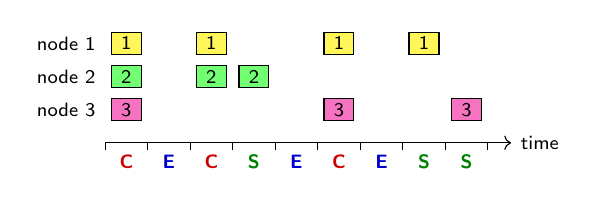
\begin{tikzpicture}[x=.54cm,y=.42cm,baseline=(current bounding box.center),
    every node/.style={font=\scriptsize}]
    % Sender rows; coincident blocks in a slot collide.
    \node[anchor=east] at (0,3) {node 1};
    \node[anchor=east] at (0,2) {node 2};
    \node[anchor=east] at (0,1) {node 3};
    \foreach \x in {0,...,9} {\draw (\x,0) -- (\x,-.22);}
    \draw[->] (0,0) -- (9.55,0) node[anchor=west] {time};
    \node[draw,fill=yellow!65,minimum width=.38cm,minimum height=.28cm,inner sep=1pt] at (.5,3) {1};
    \node[draw,fill=yellow!65,minimum width=.38cm,minimum height=.28cm,inner sep=1pt] at (2.5,3) {1};
    \node[draw,fill=yellow!65,minimum width=.38cm,minimum height=.28cm,inner sep=1pt] at (5.5,3) {1};
    \node[draw,fill=yellow!65,minimum width=.38cm,minimum height=.28cm,inner sep=1pt] at (7.5,3) {1};
    \node[draw,fill=green!55,minimum width=.38cm,minimum height=.28cm,inner sep=1pt] at (.5,2) {2};
    \node[draw,fill=green!55,minimum width=.38cm,minimum height=.28cm,inner sep=1pt] at (2.5,2) {2};
    \node[draw,fill=green!55,minimum width=.38cm,minimum height=.28cm,inner sep=1pt] at (3.5,2) {2};
    \node[draw,fill=magenta!55,minimum width=.38cm,minimum height=.28cm,inner sep=1pt] at (.5,1) {3};
    \node[draw,fill=magenta!55,minimum width=.38cm,minimum height=.28cm,inner sep=1pt] at (5.5,1) {3};
    \node[draw,fill=magenta!55,minimum width=.38cm,minimum height=.28cm,inner sep=1pt] at (8.5,1) {3};
    \node[text=red!80!black,font=\bfseries\scriptsize] at (.5,-.58) {C};
    \node[text=blue!80!black,font=\bfseries\scriptsize] at (1.5,-.58) {E};
    \node[text=red!80!black,font=\bfseries\scriptsize] at (2.5,-.58) {C};
    \node[text=green!50!black,font=\bfseries\scriptsize] at (3.5,-.58) {S};
    \node[text=blue!80!black,font=\bfseries\scriptsize] at (4.5,-.58) {E};
    \node[text=red!80!black,font=\bfseries\scriptsize] at (5.5,-.58) {C};
    \node[text=blue!80!black,font=\bfseries\scriptsize] at (6.5,-.58) {E};
    \node[text=green!50!black,font=\bfseries\scriptsize] at (7.5,-.58) {S};
    \node[text=green!50!black,font=\bfseries\scriptsize] at (8.5,-.58) {S};
  \end{tikzpicture}%
}

% IPv4 split into a subnet prefix and host ID (replaces the external PNG).
\newcommand{\ipaddressdiagram}{%
  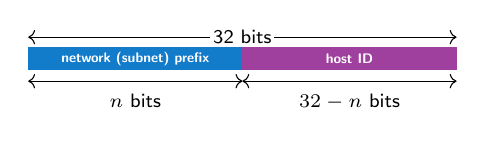
\begin{tikzpicture}[x=.17cm,y=.42cm,baseline=(current bounding box.center),
    every node/.style={font=\scriptsize}]
    \draw[<->] (0,1.35) -- (32,1.35) node[midway,fill=white,inner sep=1pt] {32 bits};
    \fill[cyan!60!blue] (0,.35) rectangle (16,1.05);
    \fill[violet!75] (16,.35) rectangle (32,1.05);
    \node[text=white,font=\bfseries\tiny] at (8,.7) {network (subnet) prefix};
    \node[text=white,font=\bfseries\tiny] at (24,.7) {host ID};
    \draw[<->] (0,.02) -- (16,.02) node[midway,below=1pt] {$n$ bits};
    \draw[<->] (16,.02) -- (32,.02) node[midway,below=1pt] {$32-n$ bits};
  \end{tikzpicture}%
}

% Embedded Ethernet preamble / start-of-frame delimiter timing waveform.
\newcommand{\preamblediagram}{%
  \resizebox{.99\linewidth}{!}{%
    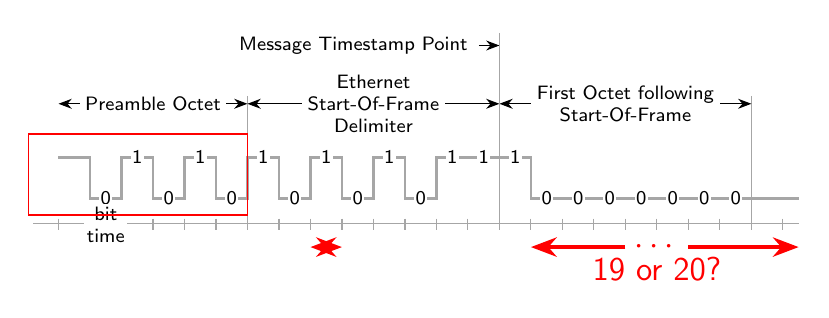
\begin{tikzpicture}[x=.40cm,y=.40cm,>=Stealth, font=\scriptsize]
      % The reference shows the last six bits of the preamble, then the SFD.
      \draw[gray!70,line width=.65pt] (-.8,-.8) -- (23.5,-.8);
      \foreach \x in {0,...,23} \draw[gray!70] (\x,-.65) -- (\x,-1.0);
      \foreach \x in {6,14,22} \draw[gray!70] (\x,3.25) -- (\x,-.8);
      \draw[gray!70,line width=1pt]
      (0,1.3) -- (1,1.3) -- (1,0) -- (2,0) --
      (2,1.3) -- (3,1.3) -- (3,0) -- (4,0) --
      (4,1.3) -- (5,1.3) -- (5,0) -- (6,0) --
      (6,1.3) -- (7,1.3) -- (7,0) -- (8,0) --
      (8,1.3) -- (9,1.3) -- (9,0) -- (10,0) --
      (10,1.3) -- (11,1.3) -- (11,0) -- (12,0) --
      (12,1.3) -- (15,1.3) -- (15,0) -- (23.5,0);
      % Place each digit on its own signal level, with white behind it.
      \foreach \x/\v/\y in {1.5/0/0,2.5/1/1.3,3.5/0/0,4.5/1/1.3,5.5/0/0,6.5/1/1.3,7.5/0/0,8.5/1/1.3,9.5/0/0,10.5/1/1.3,11.5/0/0,12.5/1/1.3,13.5/1/1.3,14.5/1/1.3,15.5/0/0,16.5/0/0,17.5/0/0,18.5/0/0,19.5/0/0,20.5/0/0,21.5/0/0} {
        \node[fill=white,inner sep=.5pt] at (\x,\y) {\v};
      }
      \draw[<->] (0,3.0) -- node[fill=white,inner sep=2pt] {Preamble Octet} (6,3.0);
      \draw[<->] (6,3.0) -- node[fill=white,inner sep=2pt,align=center]
      {Ethernet\\Start-Of-Frame\\Delimiter} (14,3.0);
      \draw[<->] (14,3.0) -- node[fill=white,inner sep=2pt,align=center]
      {First Octet following\\Start-Of-Frame} (22,3.0);
      \node[anchor=east] at (13.3,4.85) {Message Timestamp Point};
      \draw[->] (13.35,4.85) -- (14,4.85);
      \draw[gray!70] (14,5.25) -- (14,2.0);
      \node[fill=white,align=center,inner sep=1pt] at (1.5,-.85) {bit\\time};
      \draw[red,line width=.65pt] (-.95,-.52) rectangle (6,2.05);
      \draw[red,<->,line width=1.4pt] (8,-1.55) -- (9,-1.55);
      \draw[red,->,line width=1.4pt] (18,-1.55) -- (15,-1.55);
      \draw[red,->,line width=1.4pt] (20,-1.55) -- (23.5,-1.55);
      \node[red,font=\bfseries\large] at (19,-1.55) {$\cdots$};
      \node[red,font=\large] at (19,-2.25) {19 or 20?};
    \end{tikzpicture}%
  }%
}

% Black-and-white password verification flow (replaces the external PNG).
\newcommand{\passwordhashdiagram}{%
  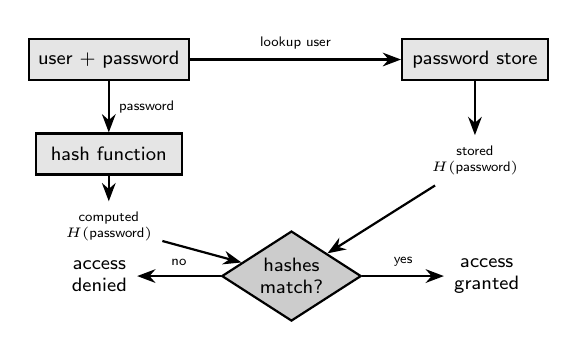
\begin{tikzpicture}[>=Stealth,font=\scriptsize,
      box/.style={draw=black,fill=black!10,minimum width=1.85cm,minimum height=.52cm,
      align=center},
      decision/.style={diamond,draw=black,fill=black!20,aspect=1.55,inner sep=1.5pt,
      align=center},
    every path/.style={->,draw=black,thick}]
    \node[box] (login) at (0,3.1) {user + password};
    \node[box] (store) at (4.65,3.1) {password store};
    \node[box] (hash) at (0,1.9) {hash function};
    \node[font=\tiny,align=center] (made) at (0,.98) {computed\\$H(\text{password})$};
    \node[font=\tiny,align=center] (saved) at (4.65,1.82) {stored\\$H(\text{password})$};
    \node[decision] (match) at (2.32,.35) {hashes\\match?};
    \node[font=\scriptsize,align=center] (deny) at (-.12,.35) {access\\denied};
    \node[font=\scriptsize,align=center] (allow) at (4.8,.35) {access\\granted};
    \draw (login) -- node[above,font=\tiny] {lookup user} (store);
    \draw (login) -- node[right,font=\tiny] {password} (hash);
    \draw (hash) -- (made);
    \draw (store) -- (saved);
    \draw (made) -- (match);
    \draw (saved) -- (match);
    \draw (match) -- node[above,font=\tiny] {no} (deny);
    \draw (match) -- node[above,font=\tiny] {yes} (allow);
  \end{tikzpicture}%
}

\begin{document}
\footnotesize % base font size for body text; tune to 8pt/9pt/tiny as needed

% ============================================================
% PAGE 1 — 4 columns
% ============================================================
\begin{multicols}{4}
  \begin{center}
    {\Large\bfseries CS2105 Cheatsheet}\\[2pt]
    Emilia Ayu
    \rule{\linewidth}{0.6pt}
  \end{center}
  \vspace{-1.5em}

  \section*{Misc. Operations}
  \sectionrule
  \subsection{Layers.}
  \begin{center}
    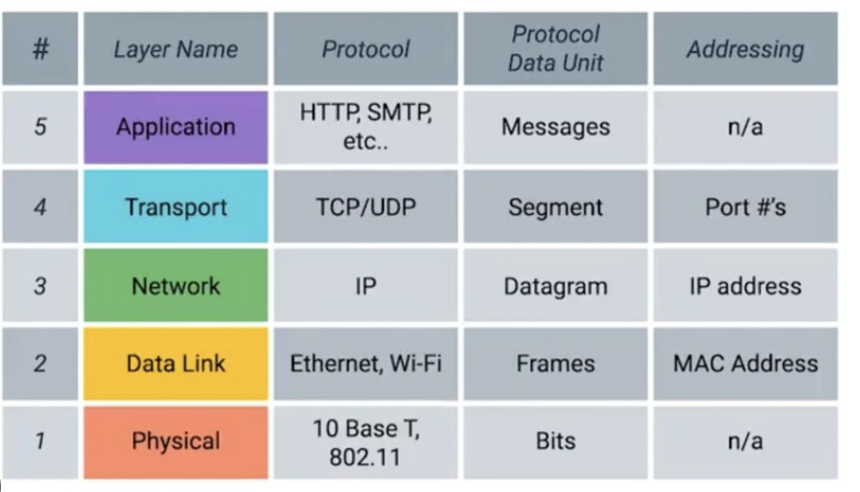
\includegraphics[width=0.75\linewidth]{misc/layers.png}
  \end{center}

  \begin{center}
    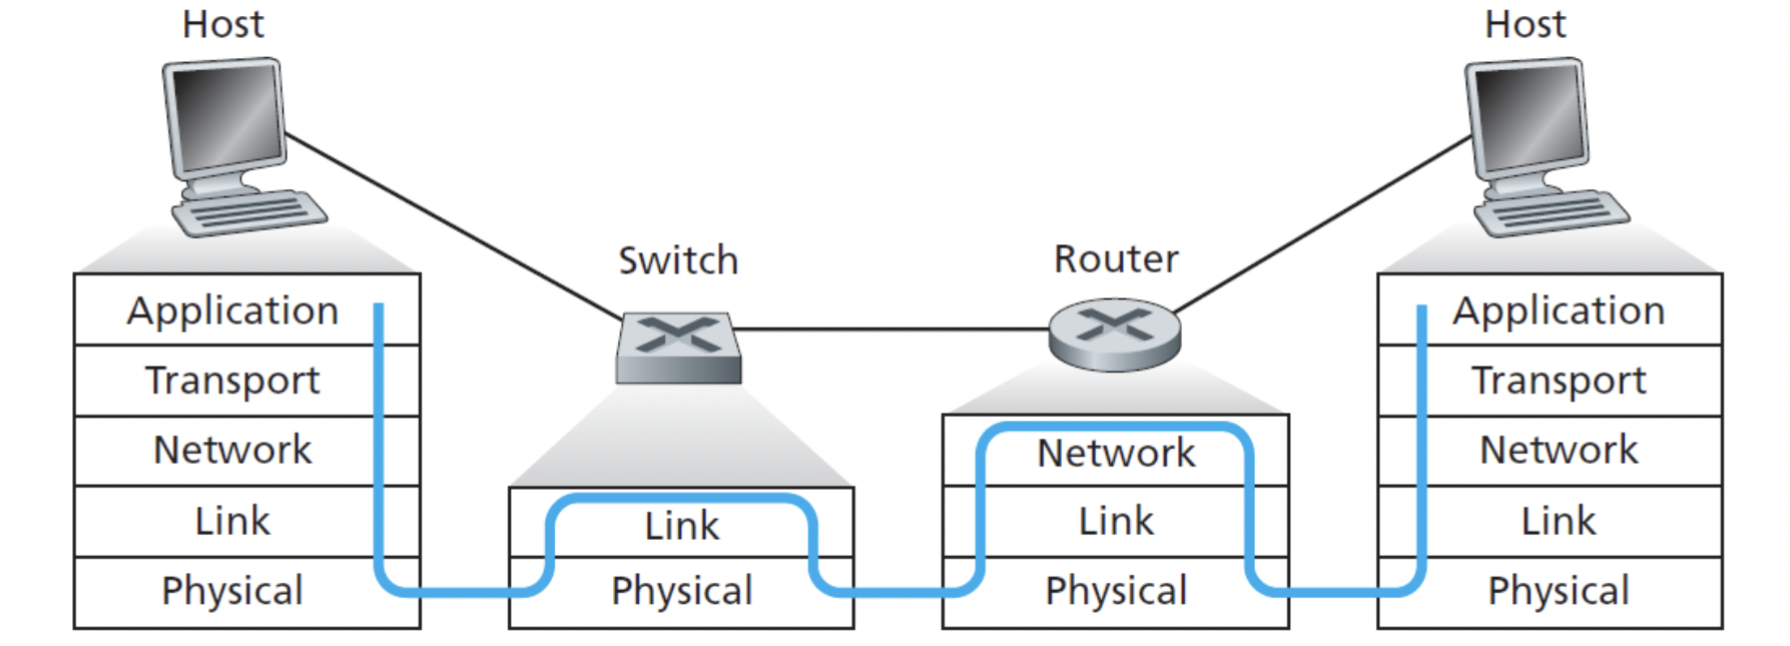
\includegraphics[width=0.75\linewidth]{misc/pipeline.png}
  \end{center}

  \subsection{Commands}
  \textbf{ping}
  Tests whether a host is reachable over a network and measures the round-trip time for packets sent to that host.

  \textbf{Usage.} \texttt{ping google.com}

  \textbf{Result.}
\begin{verbatim}
PING google.com (142.250.4.101): 56 datab
64b from IP: icmp_seq=0 ttl=102 time=17.053ms
\end{verbatim}

  \textbf{traceroute}
  Displays the sequence of routers, or network hops, that packets pass through when travelling from the source computer to a specified destination. It can be used to identify delays or failures along the route.

  \textbf{Usage.} \texttt{traceroute google.com}

  \textbf{Result.}
\begin{verbatim}
traceroute to google.com (142.250.4.101),
64 hops max
 1  192.168.1.1  2.341ms  1.872ms  1.644ms
 2  10.0.0.1   8.215ms  7.904ms  8.031ms
 3  * * *
 4  142.250.4.101  17.053ms  16.842ms  17.201ms
\end{verbatim}

  \textbf{ifconfig}
  Displays the current network configuration and status for system's first Ethernet network interface.

  \textbf{Usage.} \texttt{ifconfig eth0}
  \textbf{Result.} Contains interface status flags (whether connection is currently active (UP), capable of broadcasting (BROADCAST), or actively linked to a network (RUNNING)), IP addresses of Ethernet card, with subnet mask and broadcast address. MAC address (ether).  MTU (Maximum Transmission Unit). Shows the largest packet size (usually 1500 bytes) that the interface can transmit at once, and Packet statistics (RX and TX)

  \textbf{arp}
  Views and modifies entries in your computer's ARP cache, i.e. the local table that maps logical IP addresses (Layer 3) to physical MAC addresses (Layer 2) on LAN.
  \textbf{Usage.} \texttt{arp}

  \section*{Introduction}
  \textbf{Switching}
  \begin{itemize}
    \item \textbf{Circuit switching:} A dedicated physical path (circuit) is
      established between two nodes for the duration of the communication
      session.
    \item \textbf{Packet switching:} Data is divided into small units called
      packets.
      \begin{itemize}
        \item \textbf{Store-and-forward:} A switch must receive the entire
          packet from an incoming link before transmitting its first bit on an
          outgoing link.
      \end{itemize}
  \end{itemize}

  \textbf{Packet Loss: } Queue (aka buffer) of router has finite capacity. Packet arriving to full queue dropped

  \begin{itemize}
    \item \textit{Processing Delay: } Check bit errors, determine output link
    \item \textit{Queuing Delay: } Time waited in queue.
    \item \textit{Transmission Delay: } $\tfrac{\text{Packet length } L}{\text{Link bandwidth } R}$
    \item \textit{Propagation Delay: } $\tfrac{\text{Length of Physical link } d}{\text{Propagation speed in medium } s}$
  \end{itemize}

  \begin{center}
    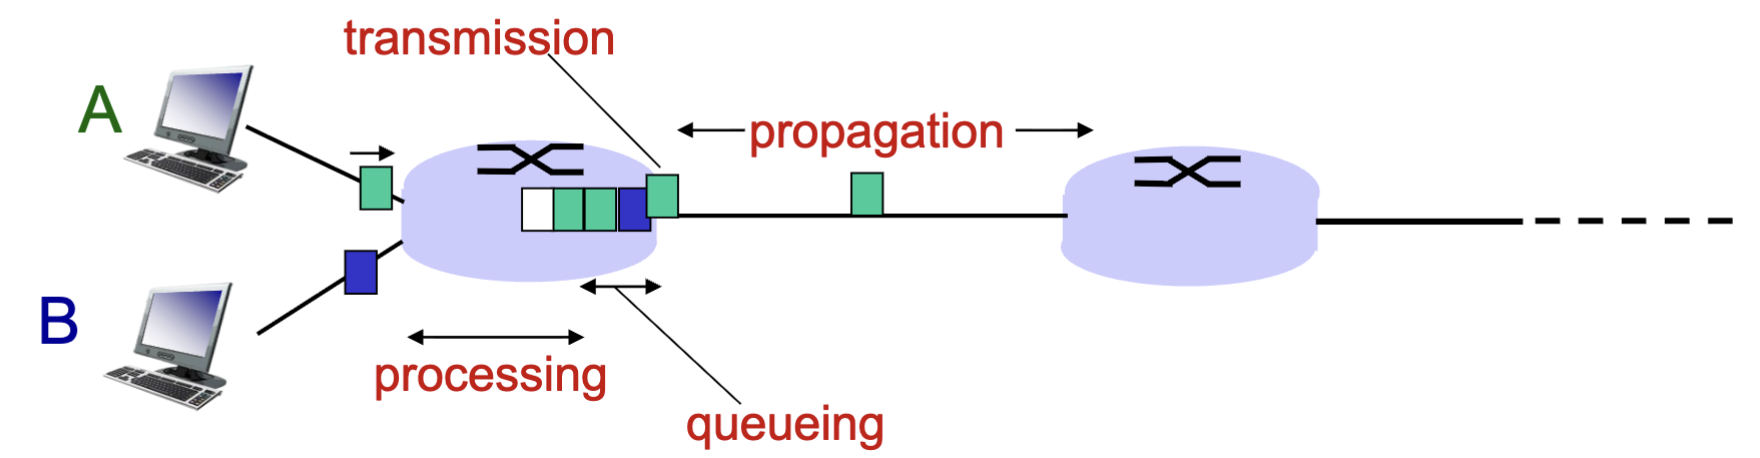
\includegraphics[width=0.75\linewidth]{application/delay-type.png}
  \end{center}
  \textit{End-to-end delay: } time taken for a packet to travel from source to destination.

  \textit{Bandwidth / link rate ($R$): } maximum rate a link can carry, in bit/s.

  \textit{Throughput ($T$): } actual rate of successfully delivered bits, in bit/s; end-to-end throughput is limited by the bottleneck link: $T \leq \min_i R_i$.

  \textit{Utilisation ($U$): } fraction of a link's bandwidth used: $U=T/R$ (multiply by $100$ for percentage).

  \section*{Layer 1 - Application Layer}
  \sectionrule

  \subsection{Network Architecture}
  \textbf{Client-Server Architecture}
  \textit{Server:} Waits for incoming requests, and provides requested service to client. Data centers for scaling
  \textit{Client:} Initiates contact with server (`speaks first'), typically requests service from server. For Web, client is usually implemented in browser

  \textbf{P2P Architecture}
  No always-on server. Arbitrary end systems directly communicate. Peers request from and provide service to from other peers. Self scalability – new peers bring new service capacity, as well as new service demands. Drawback: peers are intermittently connected and change IP addresses (complex management).

  \subsection{Web/HTTP}
  \textit{Protocols: } regulate communication activities in a network by defining the format and order of messages exchanged between hosts.
  \textit{HTTP: }Hypertext transfer protocol. Web's app layer protocol. Client/server. Uses TCP.

  \textit{RTT: }time for a packet to travel from client to server and back.
  \begin{enumerate}
    \item \textbf{Non-persistent HTTP} at most one object sent over a TCP connection (closed otherwise). Downloading multiple objects requires multiple connections. E.g. \texttt{http 1.0}
      \begin{itemize}
        \item Response Time: $2 \times RTT+ \text{file transmission time}$
      \end{itemize}
    \item \textbf{Persistent HTTP} server leaves connection open; multiple objects can be sent over single TCP connection. E.g. \texttt{http 1.1}
  \end{enumerate}

  \[
    \begin{array}{ll}
      \text{HTTP/1.0:} & \texttt{GET,\ POST,\ HEAD} \\[2pt]
      \text{HTTP/1.1:} & \texttt{GET,\ POST,\ HEAD,\ PUT,\ DELETE}
    \end{array}
  \]

  \begin{verbatim}
  HTTP/1.1 200 OK\r\n        % status line
  Date: Wed, 23 Jan 2019 13:11:15 GMT\r\n
  Content-Length: 606\r\n  % header lines
  Content-Type: text/html\r\n
  \r\n  % blank to separate headers and data
  <html>
  ...data, e.g. requested HTML file...
  </html>
  \end{verbatim}

  \textbf{Cookies: } http messages carry `state'. cookie header field of HTTP request / response messages. The cookie file is kept on user’s host, managed by user’s browser from backend

  \subsection{Domain Name System (DNS)}
  Translates hostname into IP address. Mapping is stored as resource records. Format: \texttt{<name, value, type, ttl>}. Stored in distributed databases in hierarchy of servers.
  \begin{center}
    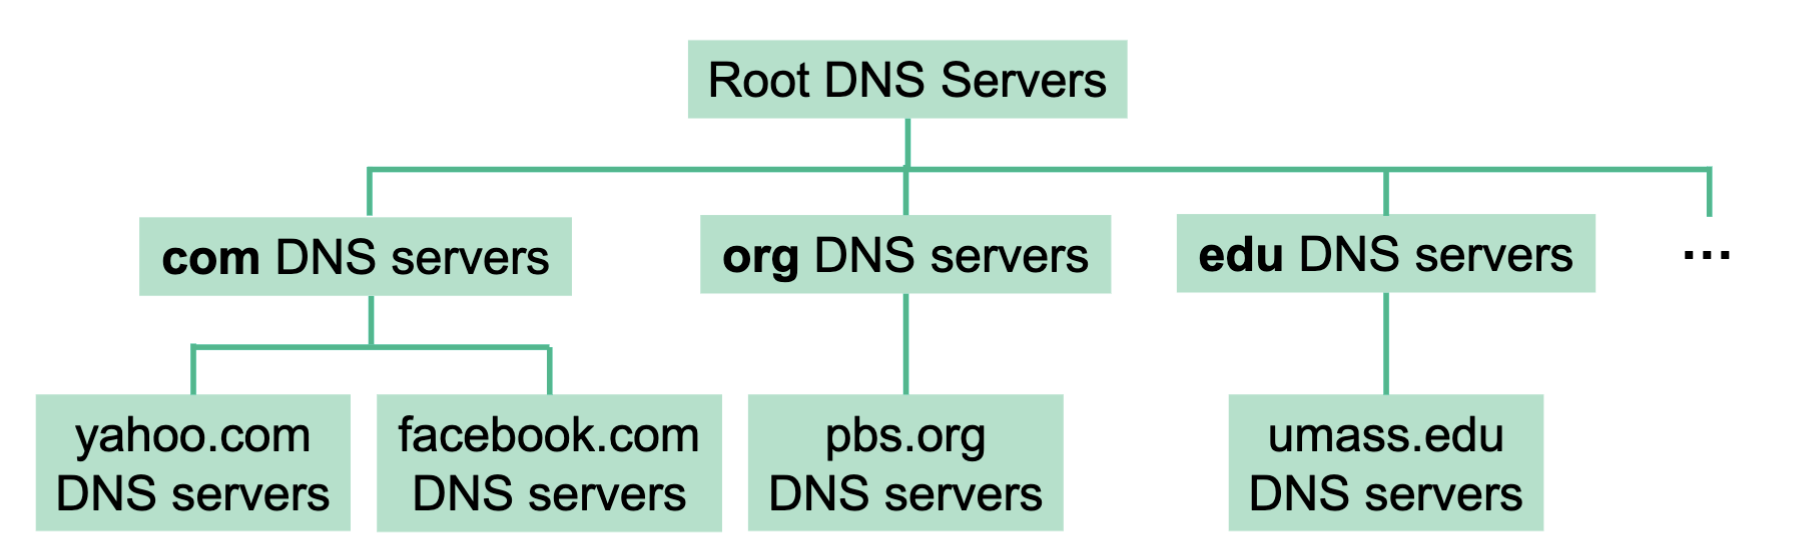
\includegraphics[width=0.75\linewidth]{application/hierarchy.png}
  \end{center}
  Servers
  \begin{enumerate}
    \item \textit{Root: } directs a query to the appropriate TLD server.
    \item \textit{Top-level domain (TLD): } \texttt{.com, .org. .edu, .sg}
    \item \textit{Authoritative: } Organization’s own DNS server
    \item \textit{Local} Each ISP (e.g. residential, school) has one local DNS server. Query is sent to local DNS server, acts as proxy and forwards query to hierarchy if not found.
  \end{enumerate}

  \textbf{DNS Caching: } Cache mapping in local DNS once learnt. Expire after TTL. Runs over UDP.

  \subsection{Dynamic Host Configuration Protocol (DHCP)}
  Application-layer protocol that leases IP configuration (e.g. IP address, subnet mask, default gateway, DNS server) when a host joins a network. Addresses can be reused after leases end. Uses UDP: client port 68, server port 67.

  \textbf{DORA:} host broadcasts \textit{Discover} $\rightarrow$ server sends \textit{Offer} $\rightarrow$ host sends \textit{Request} $\rightarrow$ server sends \textit{ACK}.

  \subsection{Socket Programming}
  \textit{Process: }program running within a host. Identified by \texttt{(IP address, port number)} (port: 16-bit). IANA coordinates assignment of port no.

  Within same host: inter-process communication (defined by OS). Different hosts: exchange messages (by protocols)

  \textbf{Socket: } software interface between app processes and transport layer protocols. TCP (\texttt{socket(AF\_INET, SOCK\_STREAM)) or UDP (socket(AF\_INET, SOCK\_STREAM)}).

  \textbf{UDP Socket Programming}
  \begin{itemize}
    \item Sender attaches dest. IP address and port no. to each packet.
    \item Receiver extracts sender IP address and port no. from received packet.
  \end{itemize}

  \textbf{TCP Socket Programming}
  \begin{itemize}
    \item Client establishes a TCP connection.
    \item Server creates a new connection socket for each client; can communicate with multiple clients separately.
    \item Server's welcome socket listens on a fixed port, e.g.\ port $80$.
  \end{itemize}

  \section*{Layer 2 - Transport Layer}
  \sectionrule
  Resides in end hosts and provides process-to-process calculation.

  \subsection{User Datagram Protocol (UDP)}
  \begin{itemize}
    \item Multiplexing at sender: UDP gathers data from processes, forms packets and passes them to IP
    \item De-multiplexing at receiver: UDP receives packets from lower layer and dispatches them to correct processes.
    \item Checksum - receiver calculates if computed checksum = checksum field value
  \end{itemize}
  Unreliable. Used by media streaming apps which are loss tolerant and rate sensitive

  \udpdiagram

  Checksum calculation:
  \begin{center}
    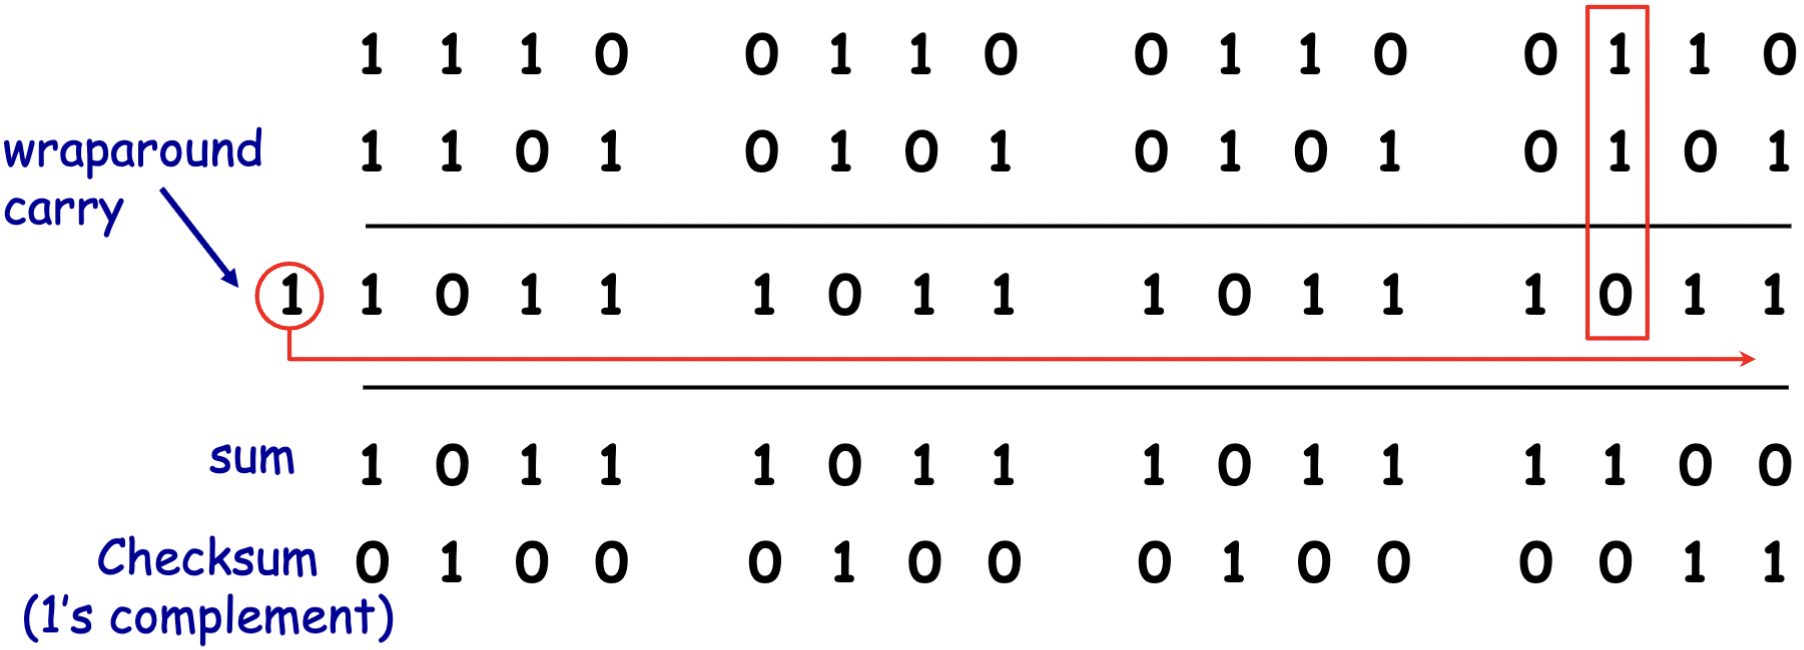
\includegraphics[width=0.75\linewidth]{transport/checksum.png}
  \end{center}

  \subsection{Reliable Data Transfer (RDT)}
Network layer has unreliable communication. Needs a reliable transport layer protocol that 1) guarantee delivery and correctness, and 2) deliver packets in the same order they are sent.

\begin{center}
\scriptsize
\setlength{\tabcolsep}{2pt}
\renewcommand{\arraystretch}{0.9}

\resizebox{\columnwidth}{!}{%
  \begin{tabular}{lccccc}
    \hline
    \textbf{RDT} &
    \textbf{Checksum} &
    \textbf{ACK} &
    \textbf{NAK} &
    \textbf{Seq. no.} &
    \textbf{Timer} \\
    \hline
    \texttt{1.0} & \texttimes & \texttimes & \texttimes & \texttimes & \texttimes \\
    \texttt{2.0} & \checkmark & \checkmark & \checkmark & \texttimes & \texttimes \\
    \texttt{2.1} & \checkmark & \checkmark & \checkmark & \checkmark & \texttimes \\
    \texttt{2.2} & \checkmark & \checkmark & \texttimes & \checkmark & \texttimes \\
    \texttt{3.0} & \checkmark & \checkmark & \texttimes & \checkmark & \checkmark \\
    \hline
  \end{tabular}%
}
\end{center}

\begin{itemize}
\item \texttt{rdt1.0}: assumes reliable channel. no error.
\item \texttt{rdt2.0}: handles bit errors; corrupted ACKs/NAKs cannot be recovered.
\item \texttt{rdt2.1}: use sequence numbers to discard duplicates.
\item \texttt{rdt2.2}: no NAKs; send prev ACK. Duplicate indicates error.
\item \texttt{rdt3.0}: handles packet loss with timer (if packet is delayed). Retransmit when timeout.
\end{itemize}

\textbf{rdt 3.0 Stop and Wait}
\[
U_{\mathrm{s}}=\frac{L/R}{RTT+L/R}
\]
\textit{Low utilisation; ignore ACK transmission and processing time.}
\begin{center}
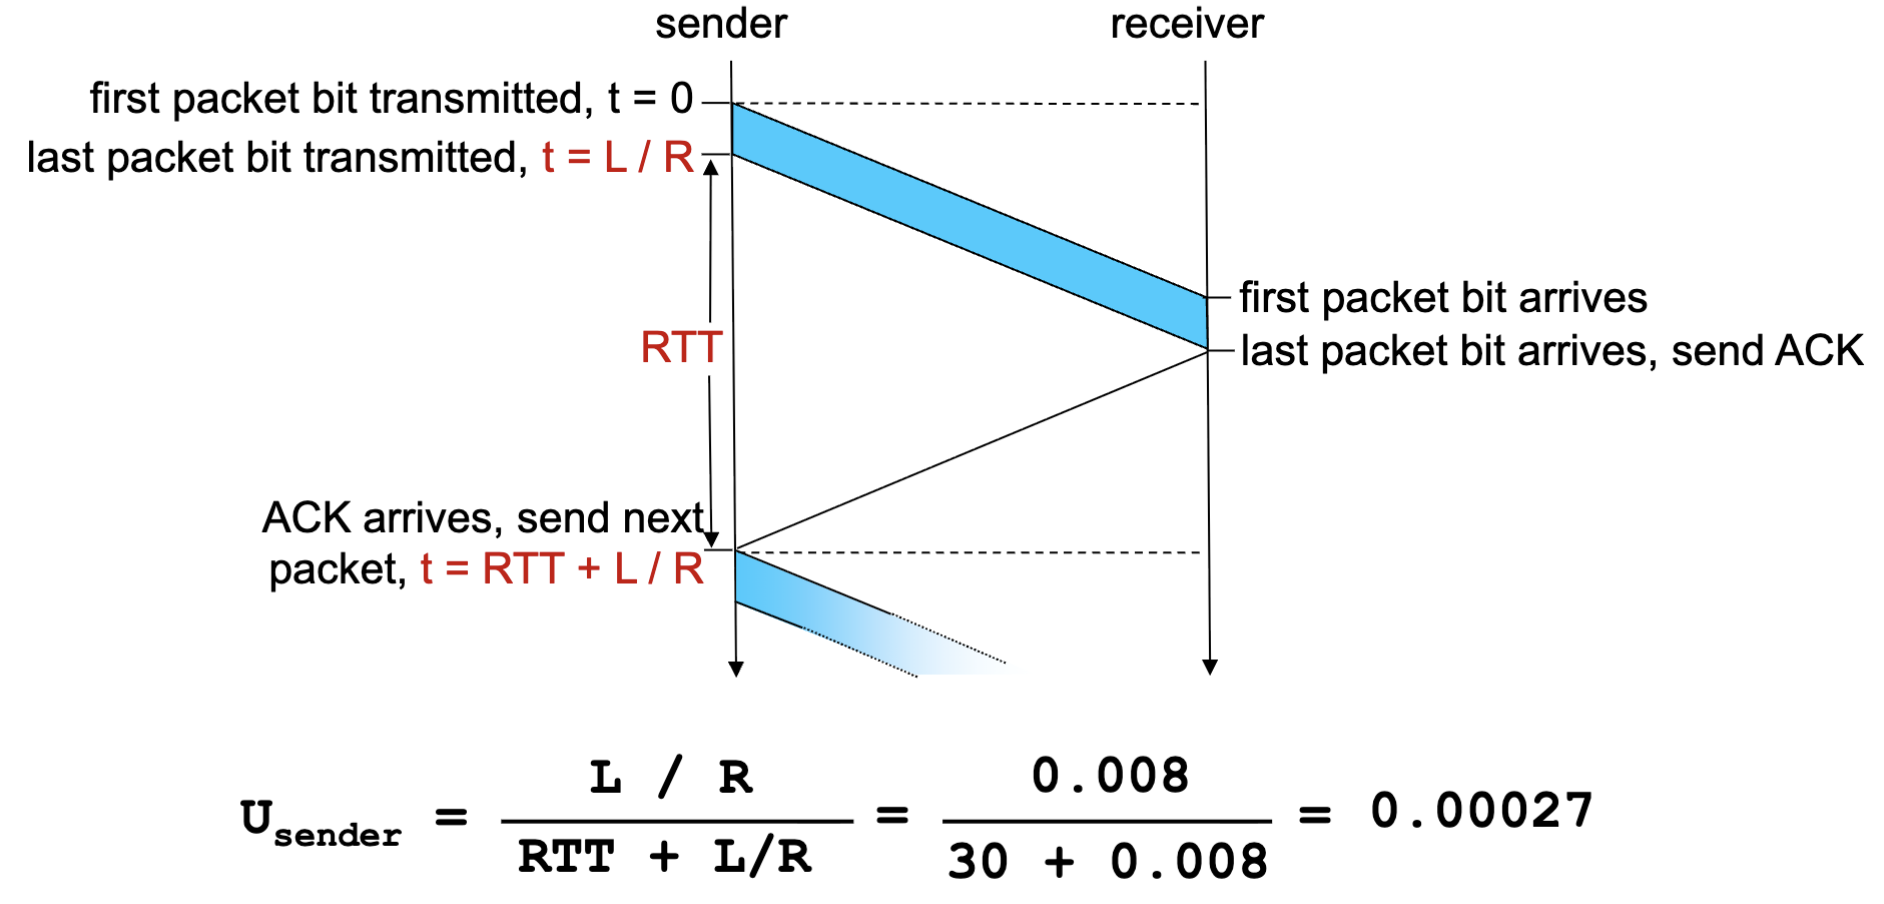
\includegraphics[width=0.75\linewidth]{transport/stop-wait.png}
\end{center}

\subsection{Pipelined Protocols}
\textbf{Go Back N} uses cumulative ACK - `ACK m' means all packets up to m are received. Receiver only ACKs packets arriving in order. Sender uses sliding window to keep track of unACK-ed packet, and timer for oldest unACK-ed.
\begin{center}
\gobackndiagram
\end{center}

\textbf{Selective Repeat} Receiver individually acknowledges all correctly received packets. Buffer out-of-order packets. Sender maintains timer for each unACKed packet. Retransmit only that packet upon timeout.

\begin{center}
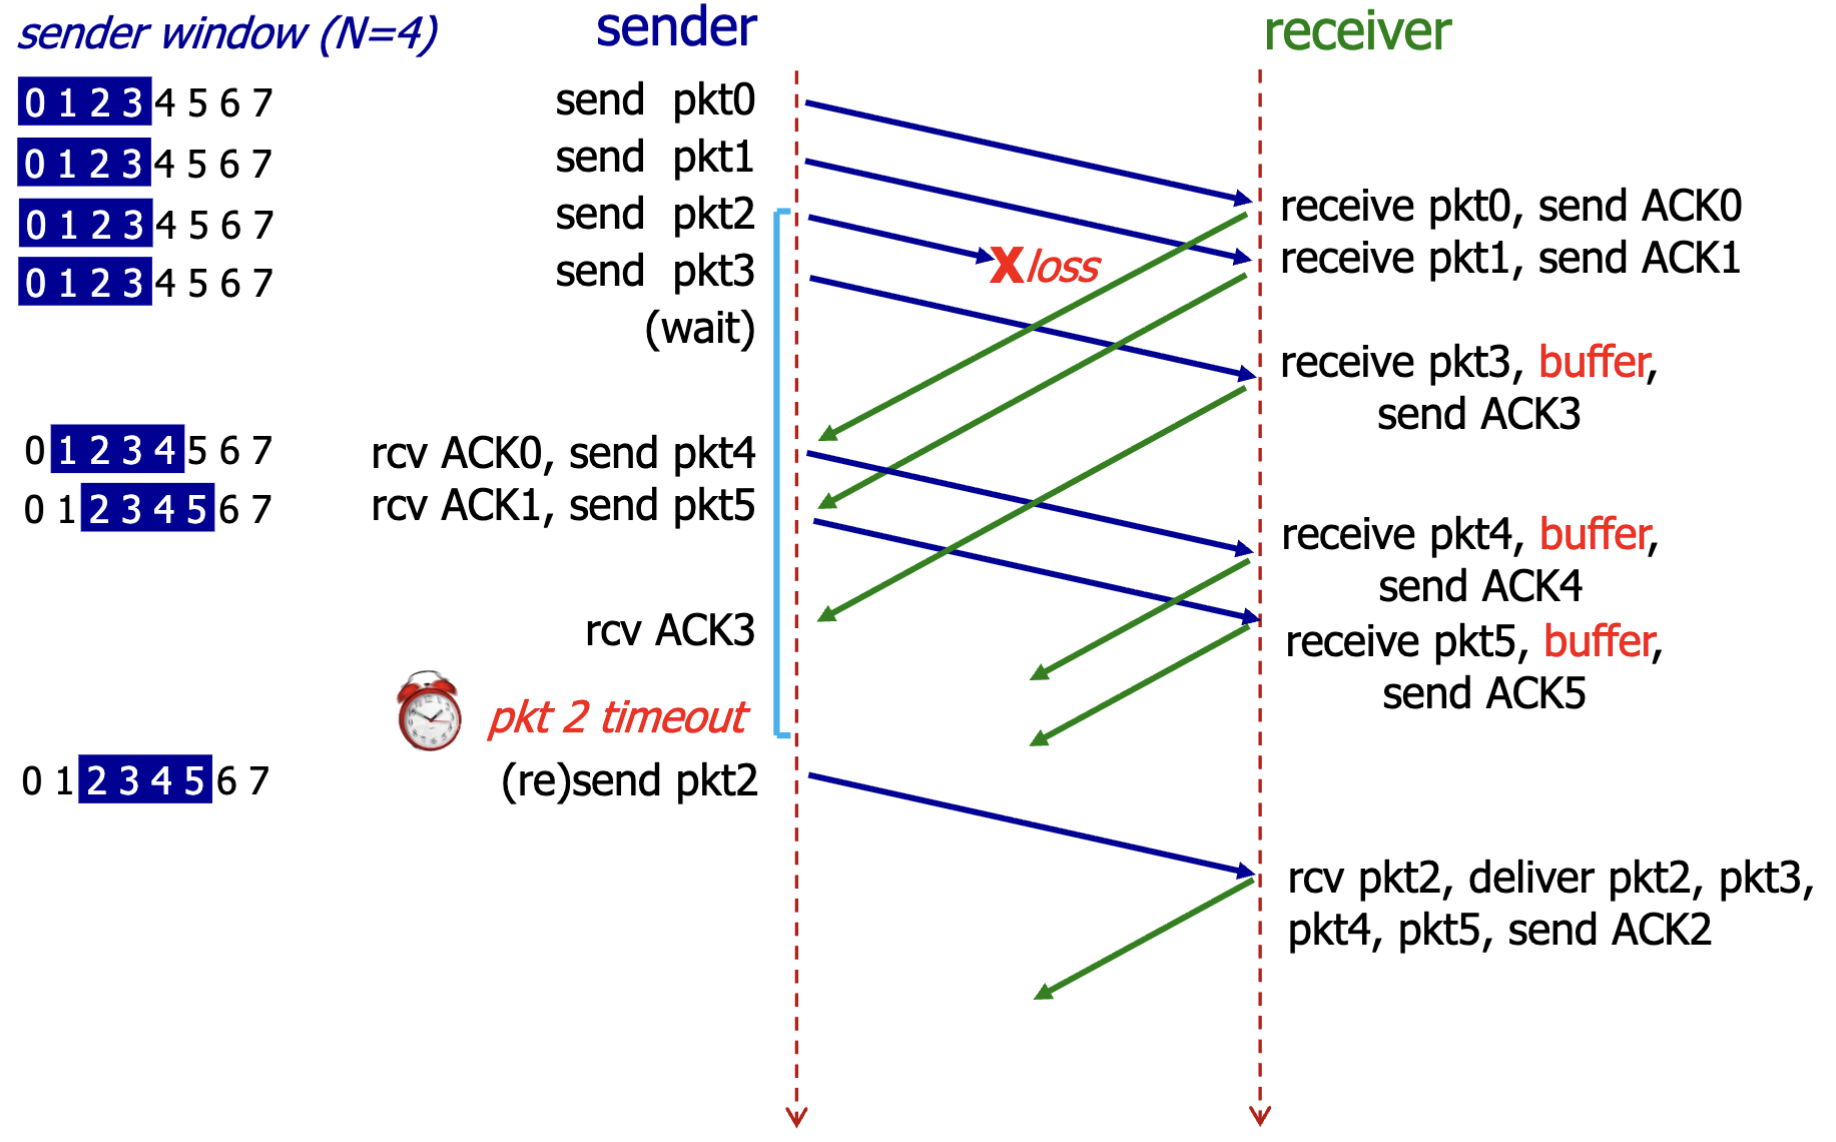
\includegraphics[width=0.75\linewidth]{transport/selective-repeat.png}
\end{center}

\subsection{Transmission Control Protocol (TCP)}
Connection: \texttt{<srcIPAddr, srcPort, destIPAddr, destPort>}
TCP send and receive buffers, created after handshaking at any side. Each TCP segment can carry Maximum Segment Size (MSS) in app-layer data.

TCP Segment Structure
\begin{center}
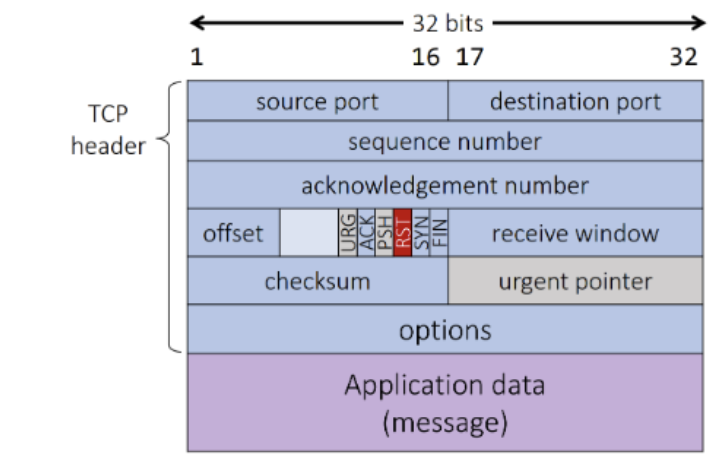
\includegraphics[width=0.75\linewidth]{transport/tcp-struct.png}
\end{center}
\textit{Seq. no.: } first byte of data in a segment. \textit{ACK no.: } Seq \# of the next byte of data expected by receiver.

\begin{center}
\scriptsize
\setlength{\tabcolsep}{2pt}
\renewcommand{\arraystretch}{0.75}

\begin{tabular}{ccc}
  \hline
  \textbf{Segment seq.} & \textbf{Data carried} & \textbf{ACK number} \\
  \hline
  0       & 1{,}000 & 1{,}000 \\
  1{,}000 & 1{,}000 & 2{,}000 \\
  \hline
\end{tabular}
\end{center}

TCP (and also UDP) is a full duplex protocol - bi-directional data flow in the same TCP connection.

\begin{center}
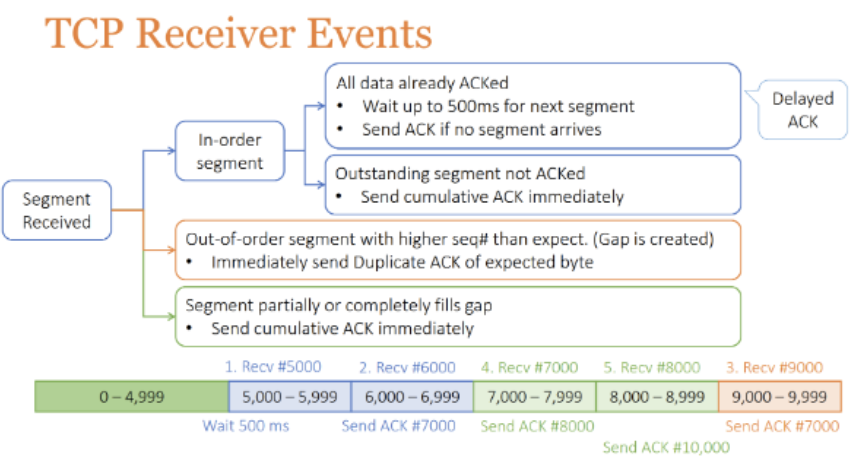
\includegraphics[width=0.75\linewidth]{transport/tcp-receiver.png}
\end{center}

\textbf{TCP Timeout Interval} TCP continuously updates timeout interval based on estimated RTT.

$\text{Est.RTT} = (1-\alpha)\text{Est.RTT} +\alpha\text{SampleRTT}$,\\
$\text{DevRTT} = (1-\beta)\text{DevRTT} +\beta\left|\text{SampleRTT} \text{Est.RTT}\right|$,\\
$\text{TimeoutInterval} = \text{Est.RTT}+4\text{DevRTT}$

\textbf{TCP Handshake}
\textit{Establishing Connection}

\begin{center}
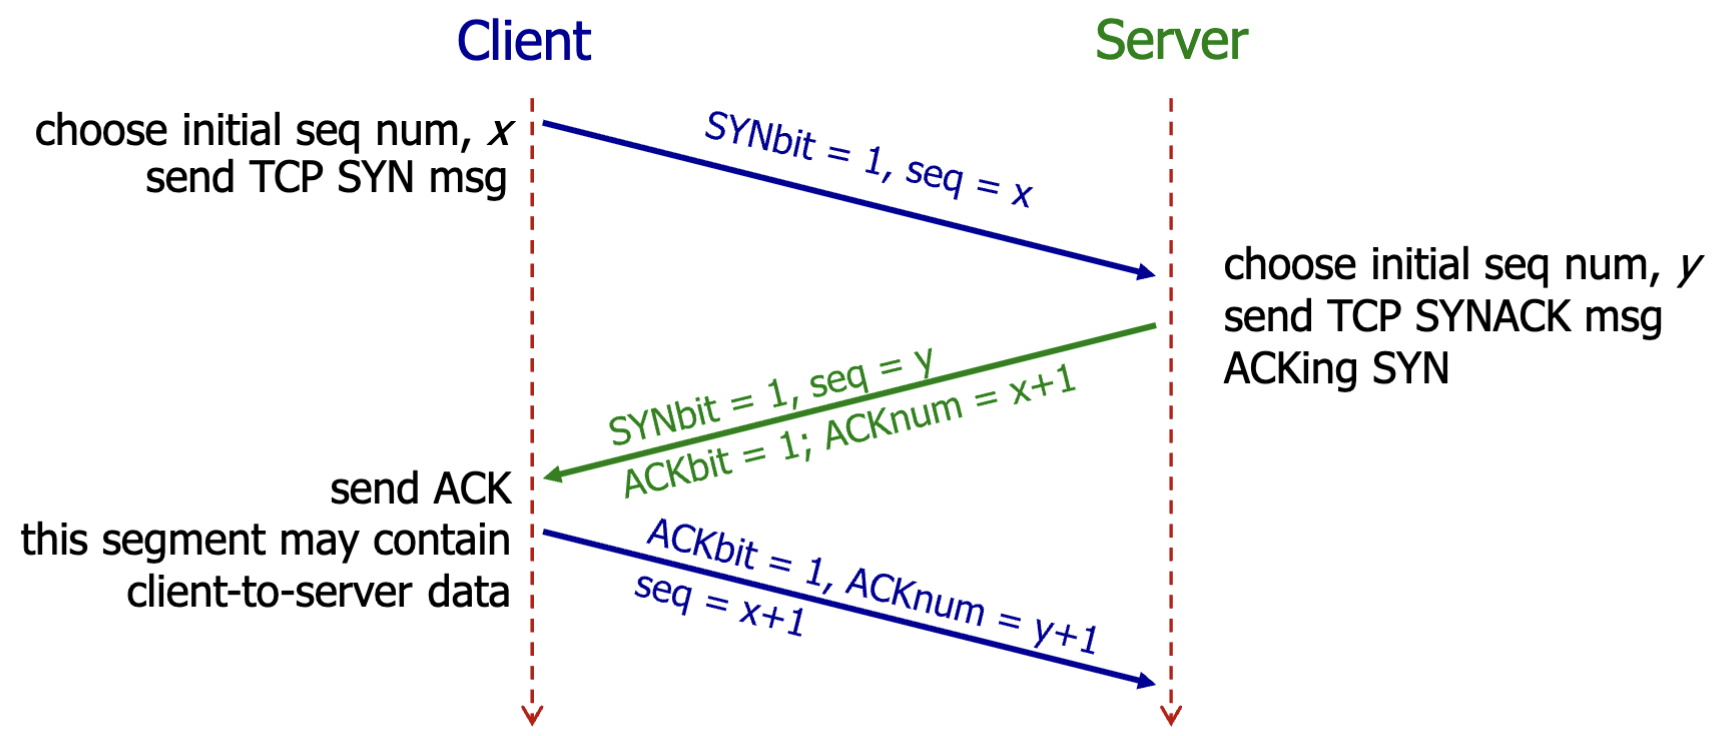
\includegraphics[width=0.75\linewidth]{transport/handshake-open.png}\\[0.5em]
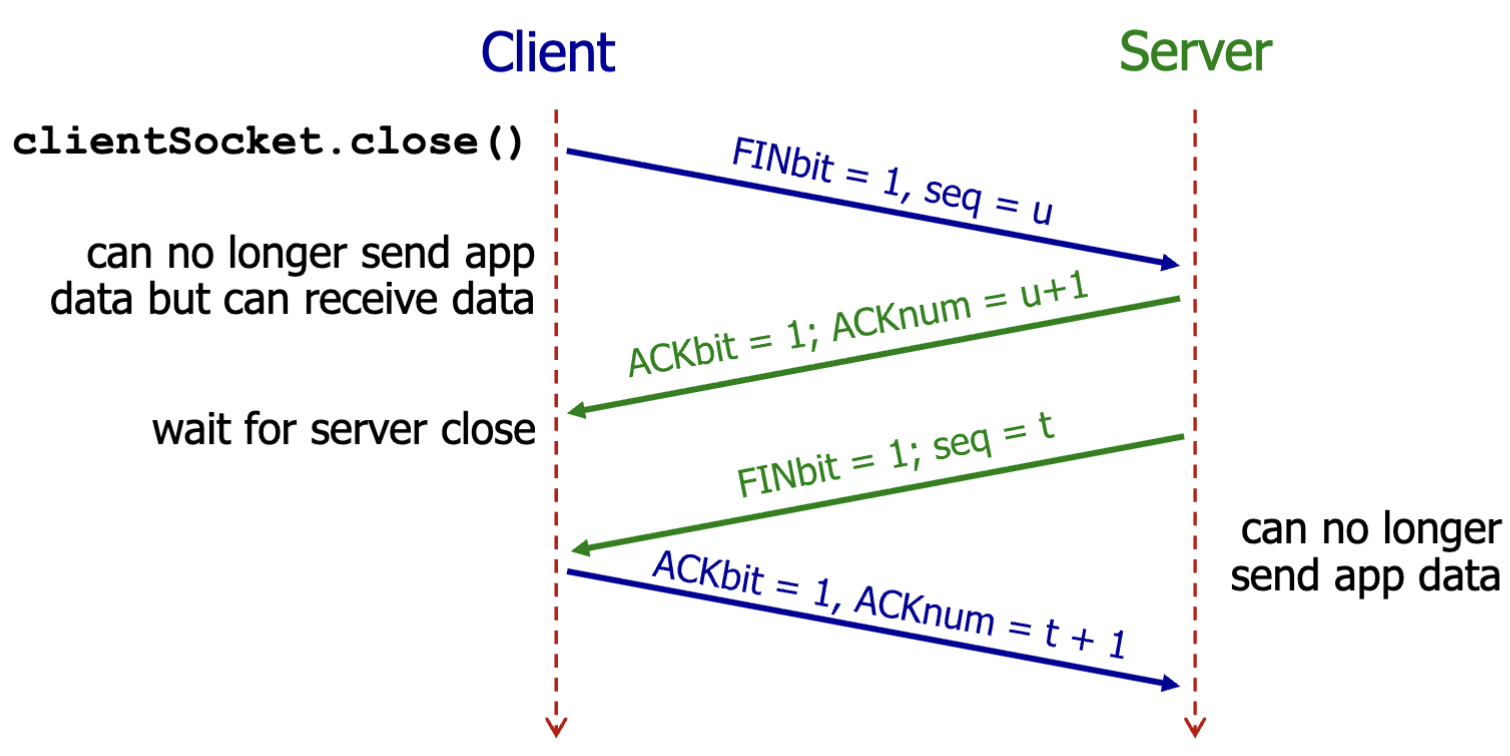
\includegraphics[width=0.75\linewidth]{transport/handshake-close.png}
\end{center}

\section*{Layer 3 - Network Layer}
\sectionrule
The network layer delivers packets to receiving hosts

\subsection{IP Address} Used to identify a host (or a router).
A host gets an IP addr. either by:
\begin{enumerate}
\item manually configured by system administrator, or
\item automatically leased by a DHCP server.
\end{enumerate}

\begin{center}
\ipaddressdiagram
\end{center}
For CIDR \texttt{a.b.c.d/$n$}: host bits $=32-n$;
\textbf{total addresses} $=2^{32-n}$. Normally usable host addresses
$=2^{32-n}-2$: the address with all host bits 0 is the \emph{network ID},
and the one with all host bits 1 is the \emph{directed broadcast}, so neither
is assigned to a host. (/31 point-to-point links and /32 host routes are
exceptions.)

\paragraph{Special IP Addresses.}
\begin{center}
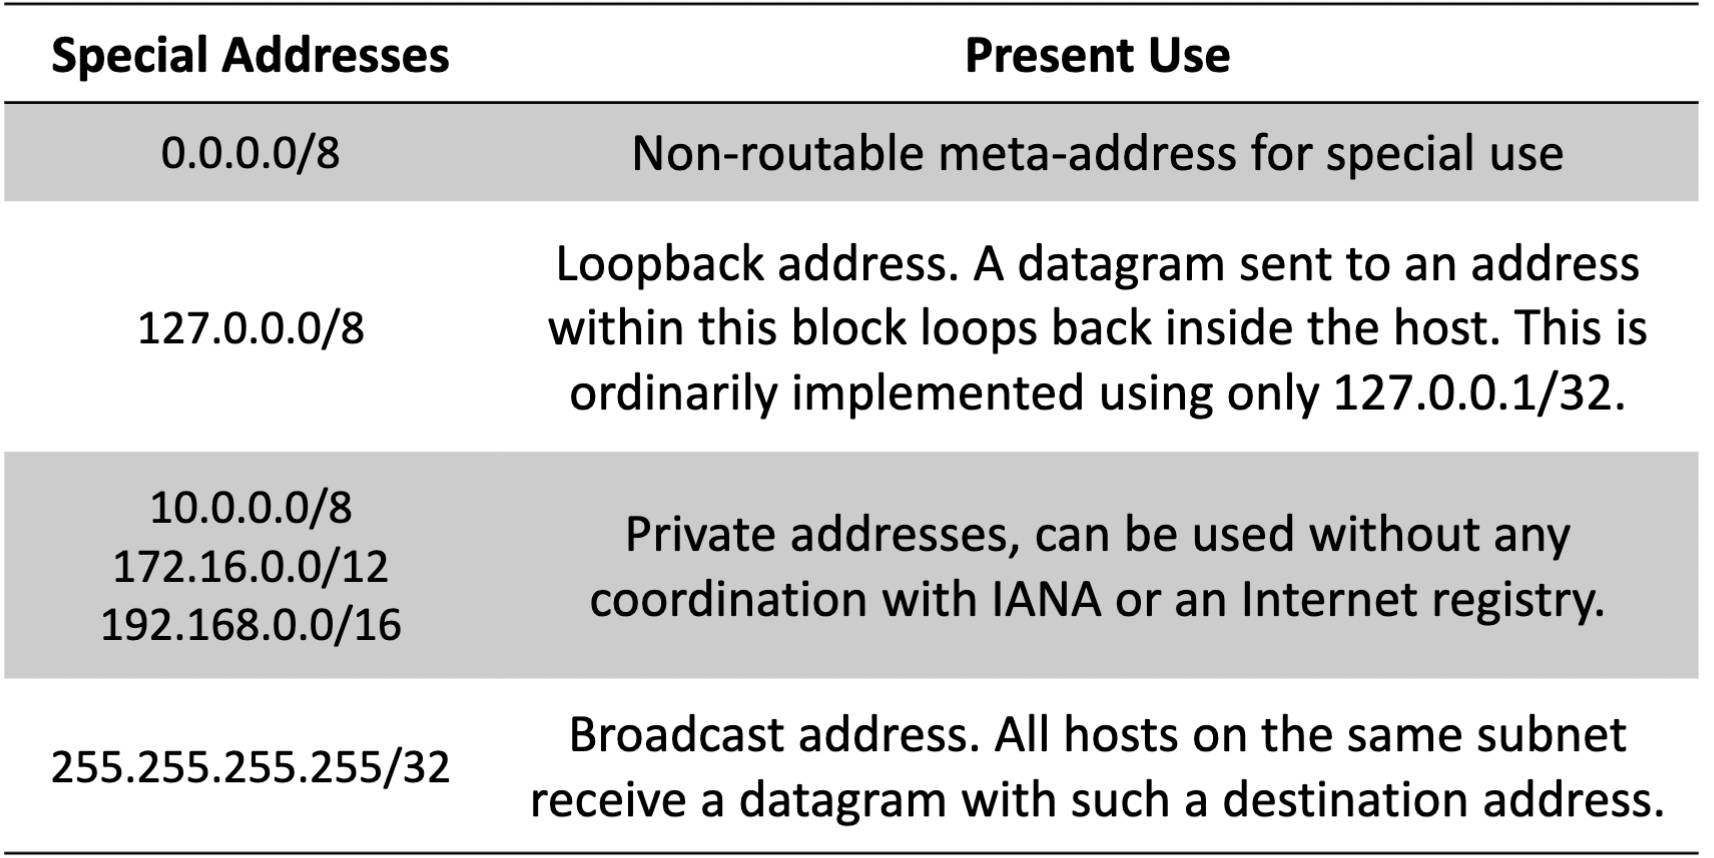
\includegraphics[width=0.75\linewidth]{network/special.png}
\end{center}

\textbf{IP Fragmentation.} A fragment has its own IP header, a shared
Identification value, a Fragment Offset (in 8-byte units), and the More
Fragments flag. When a TCP segment is fragmented, only the first fragment
contains the TCP header; later fragments carry payload. Reassembly is at the
final destination.

\textbf{Subnet.} A network formed by a group of “directly” interconnected hosts. Hosts in the same subnet have the same network prefix of IP address. Can reach each other without router.

\textbf{Classless Inter-domain Routing (CIDR).} Internet's IP Address assigning strategy.
Address format: \texttt{a.b.c.d/x}, where \texttt{x} is the number of bits in subnet prefix.

Subnet mask determines which subnet an IP address belongs to. Set all subnet bits t 1 and host id bits to 0.

\textbf{Hierarchical addressing} uses subnet masks to structure addresses into blocks. Pros are upstream routers do not need to know every single individual host or minor subnet.
\textbf{Longest prefix match} compares dest. IP address against every entry in forwarding table and returns one with the longest matching subset mask.

An ISP get a block of addresses from ICANN: Internet Corporation for Assigned Names and Numbers. Allocates addresses, manages DNS, and assigns domain names.

\subsection{Routing Algorithms}
Intra-AS routing. Find a good path between two routers within an AS (autonomous system, e.g. ISPs). Single admin, so no policy decisions are needed and routing focuses on performance.

$$d_x(y) = \min_v{c(x, v), d_v(y)}$$
where $c(x, y)$ is the cost of link between routers x and y, infinity if x and y are not direct neighbours, and $d_x(y)$ is the cost of the least-cost path from x to y from x’s view.

\textbf{Distance Vector Algorithms}
Every router, x, y, z, sends its distance vectors to its directly connected neighbors.
When x finds out that y is advertising a path to z that is cheaper than x currently knows, x will update its distance vector to z accordingly. x will note down that all packets for z should be sent to y. Update forwarding table of x
After every router has exchanged several rounds of updates with its direct neighbors, all routers will know the least-cost paths to all the other routers.

\textbf{Routing Information Protocol (RIP)} implements the DV algorithm. Uses hop count as the cost metric (i.e., insensitive to network congestion).
Exchange routing table every 30 seconds over UDP port 520.
“Self-repair”: if no update from a neighbour router for 3 minutes, assume neighbour has failed

\textbf{IPv4 Datagram.}
\begin{center}
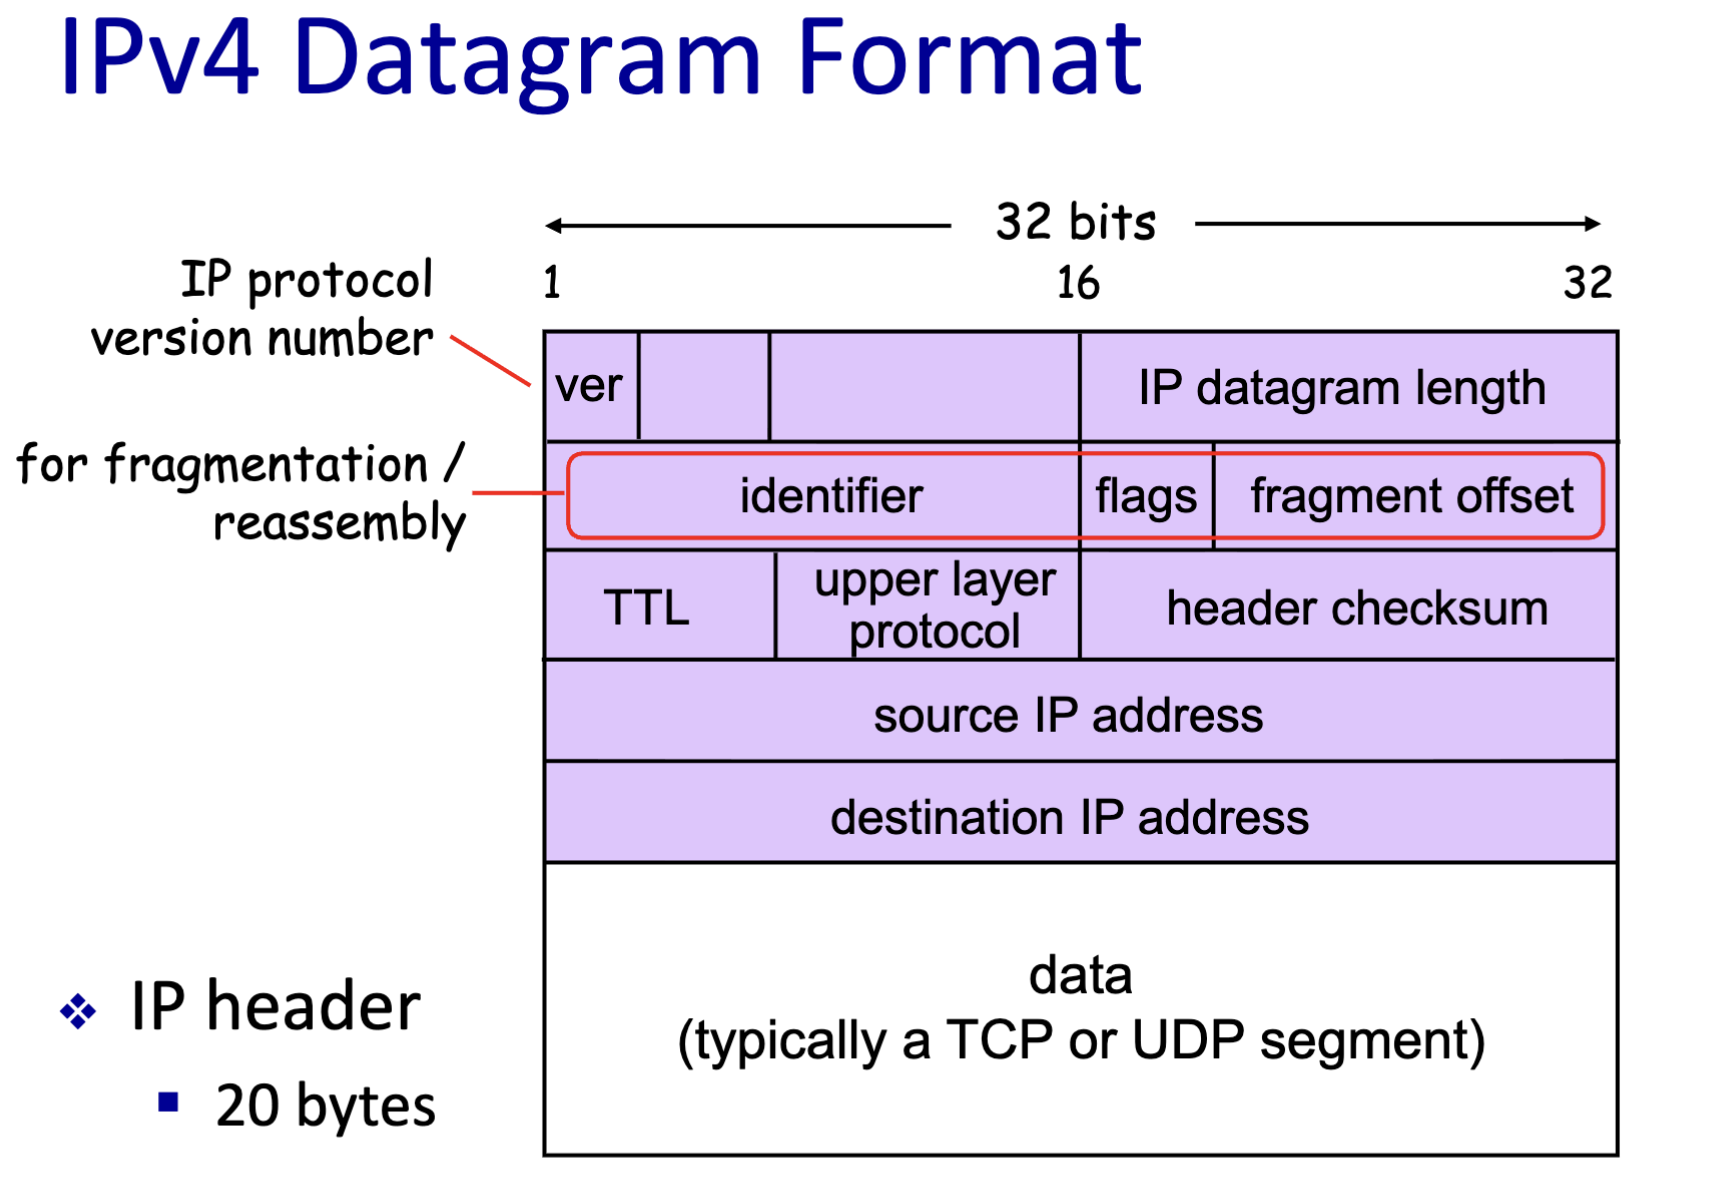
\includegraphics[width=0.75\linewidth]{network/ipv4.png}
\end{center}

\subsection{Network Address Translation (NAT)}
Maps one IP addresses space into another
\begin{center}
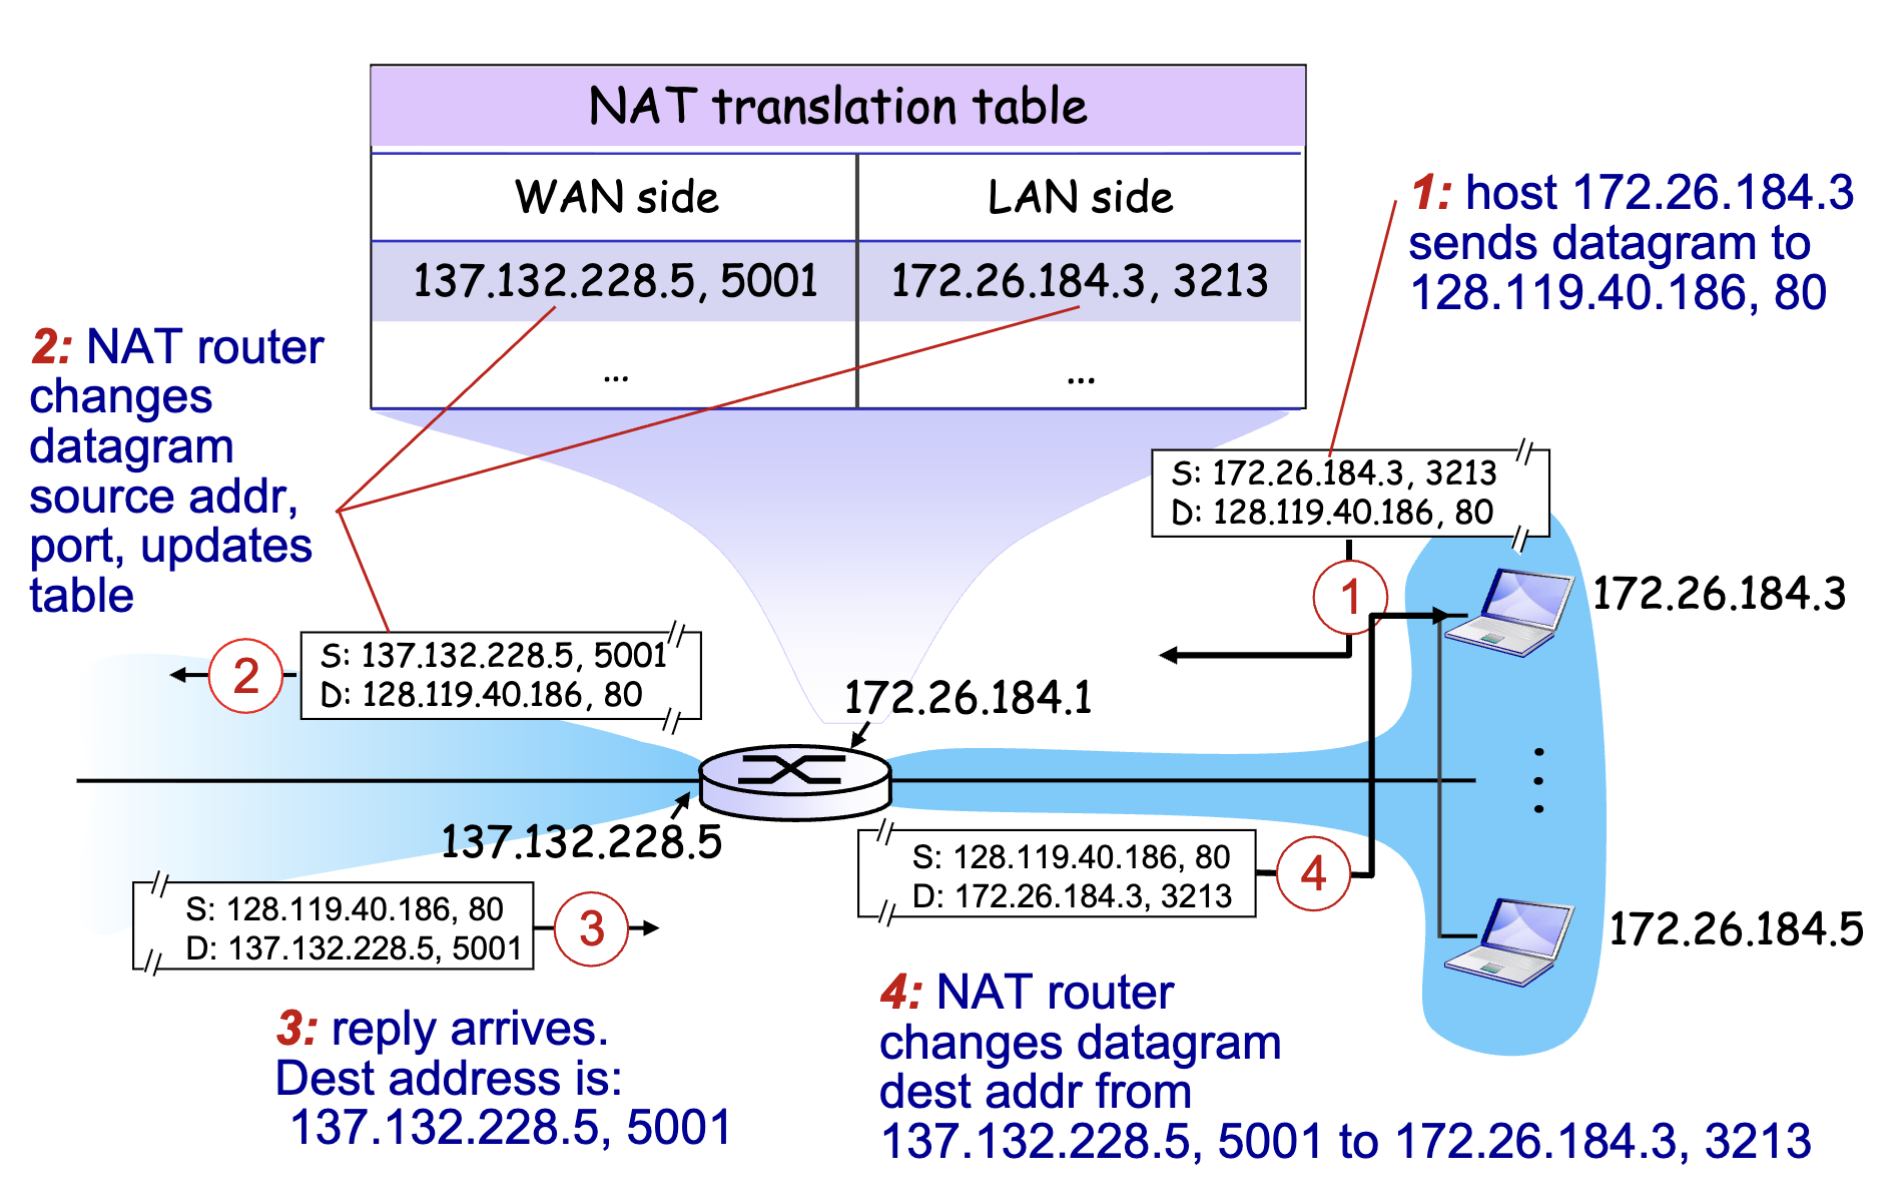
\includegraphics[width=0.75\linewidth]{network/nat.png}
\end{center}
\begin{itemize}
\item Replace (source IP address, port \#) of every outgoing datagram to (NAT IP address, new port \#).
\item Remember (in NAT translation table) the mapping from (source IP address, port \#) to (NAT IP address, new port \#).
\item Replace (NAT IP address, new port \#) in destination fields of every incoming datagram with corresponding (source IP address, port \#) stored in NAT translation table
\end{itemize}

\textbf{Benefits.} Only need one public IP for the NAT router. All hosts use private IP addresses so addresses of hosts can be changed in local network without notifying outside.
Can change ISP without changing addresses of hosts
in local network. Hosts inside local network are not explicitly addressable and visible by outside world (security).

MTU (Max Transfer Unit) the maximum amount of data a link-level frame can carry.

\subsection{Internet Control Message Protocol}

Used by hosts \& routers to communicate network-level
information. E.g. error reporting: unreachable host / network / port / protocol and echo request/reply (used by \texttt{ping})

\begin{center}
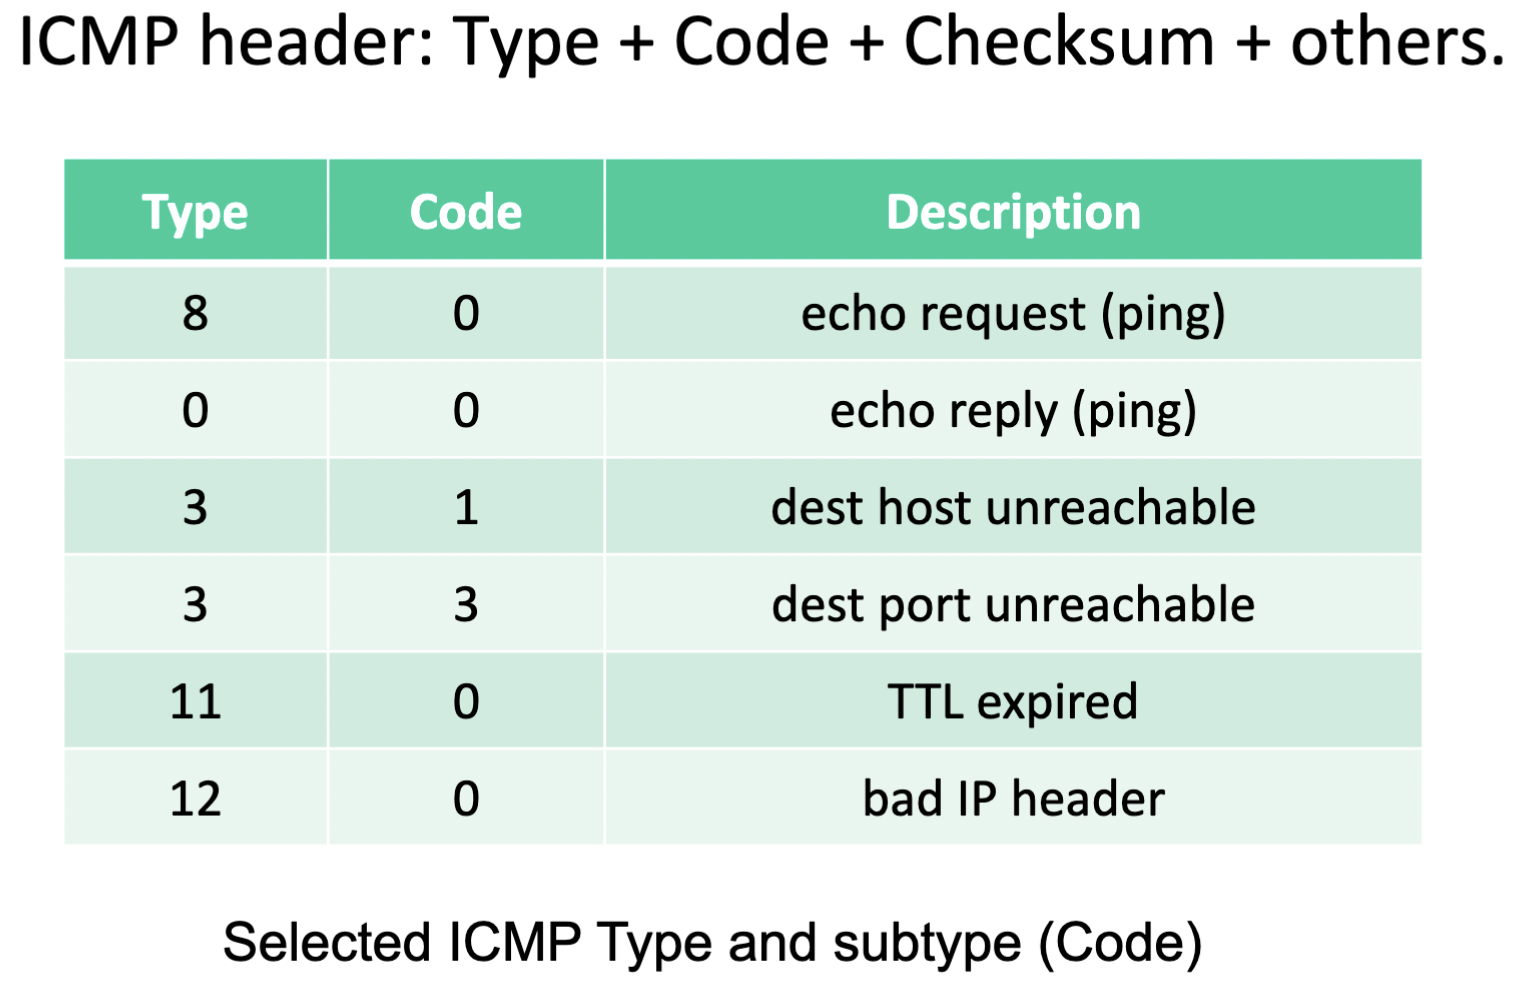
\includegraphics[width=0.75\linewidth]{network/icmp-type.png}
\end{center}

\section*{Layer 4 - Link Layer}
\sectionrule
Sends datagram between adjacent nodes (hosts or routers) over a single link. IP datagrams are encapsulated in link-layer frames for transmission
Link layer has responsibility of transferring datagram from one node to physically adjacent node over a link.

\textbf{Communication channel: } the transmission medium of the data signals. E.g. copper wire, optical fiber, terrestrial radio, Satellite. \\
\textbf{Nodes: } Devices exchanging data. e.g. hosts, routers
\textbf{Adjacent: } Single hop connects the two nodes
\textbf{Frame: } Layer-2 packet

Implemented in adapter eg NIC (Network Interface Card)

Link Layer Services.
\begin{enumerate}
\item \textbf{Framing: } encapsulate data into a frame, add header and trailer
\item \textbf{Link Access Control: } When multiple nodes share a single link, coordinate which nodes can send frames at each point of time
\item \textbf{Error detection}
\item \textbf{Error correction}
\item \textbf{Reliable delivery: } often used on error-prone delivery like wireless link.
\end{enumerate}

\subsection{Multiple Access Links and Protocols}

\textbf{Types of Network Link}
\begin{itemize}
\item \textbf{Type 1: point-to-point link} A sender and a receiver connected by a dedicated link (eg host to router). Use protocols Point-to-Point Protocol (PPP), Serial Line Internet Protocol (SLIP). No need multiple access.
\item \textbf{Type 2: broadcast link } Multiple nodes connected to a shared broadcast channel. When a node transmits a frame, the channel broadcasts the frame and every other node receives a copy. If two or more nodes transmit simultaneously, it leads to a \textbf{collision}
\end{itemize}

\textbf{Given}: Broadcast channel of rate R bps
Desired Properties:
\begin{enumerate}
\item Collision Free
\item Efficient: when only one node wants to transmit, it can send at rate R.
\item Fairness: when M nodes want to transmit, each can send at same average rate R/M (approx.)
\item fully decentralized, i.e. no special node to coordinate transmissions
\end{enumerate}

coordination about channel sharing must use channel itself!: no out-of-band channel signaling

\subsection{Random Access Protocols}
Random access protocols specify how to detect collisions and how to recover from collisions

\textbf{Slotted ALOHA}
When node has data to send transmit at full channel data rate $R$, and no a priori coordination among nodes. Data sent in frames of size $L$ bits.
\begin{itemize}
\item Time divided into synchronized slots of duration \(L/R\).
\item Nodes transmit at the start of the next slot when they have a frame.
\item After a collision, retransmit in each subsequent slot with probability \(p\).
\end{itemize}
\begin{center}
\slottedalohadiagram
\end{center}

\textbf{Unslotted ALOHA}
No time slots, no synchronisation. When fresh frame:
\begin{itemize}
\item Transmits the entire frame immediately.
\item If no collision: data transmission is a success.
\item If collision: data transmission is a failure. Wait for 1 frame transmission time, retransmit in each subsequent slot with probability \(p\)
\item Chance of collision increases.
\end{itemize}

\begin{center}
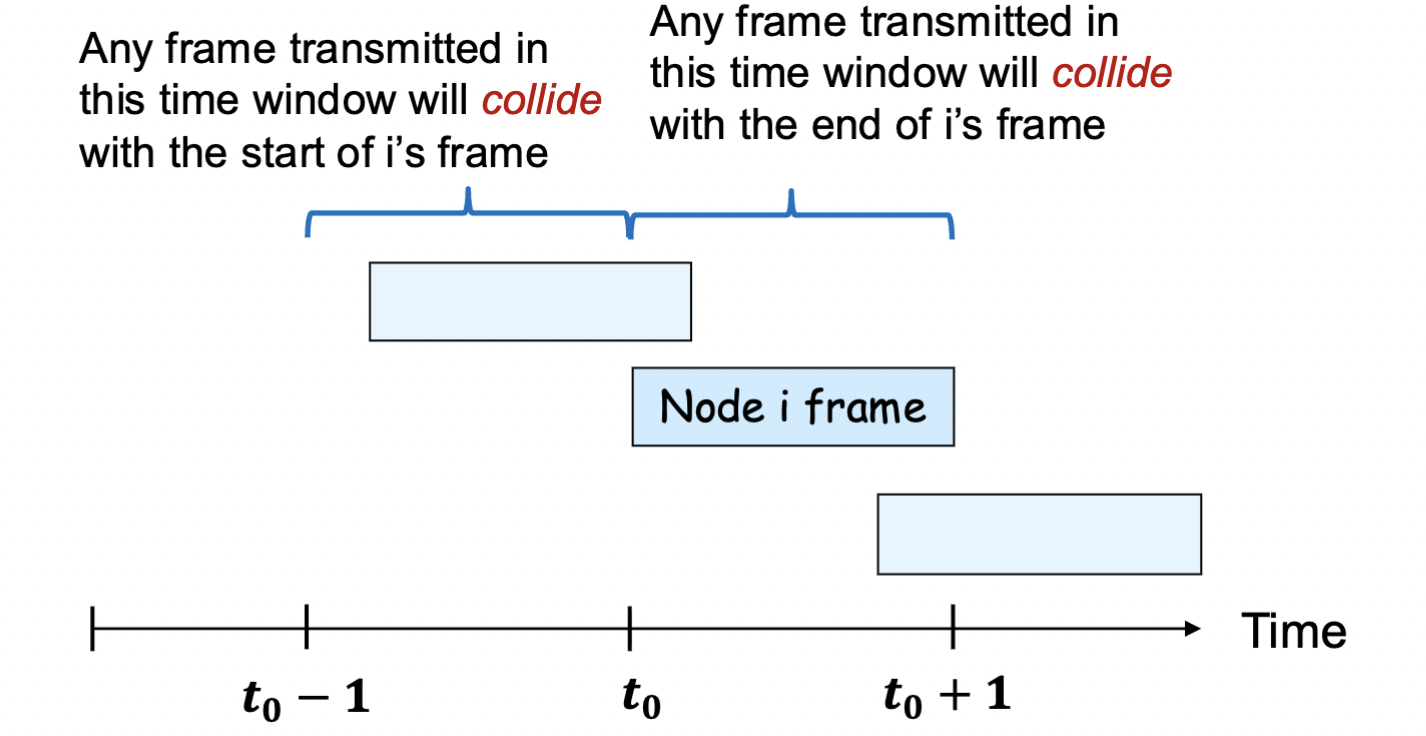
\includegraphics[width=0.75\linewidth]{link/unslotted-aloha.png}
\end{center}

\textbf{Limitations of both ALOHAs: } node’s decision to transmit is independent of the activity of other nodes in broadcast channel, and node pays no attention to whether another node is transmitting

\textbf{Carrier Sense Multiple Access}
Listen before transmit. If channel idle, transmit, else defer transmission.
Possible collision from propagation delay

\textbf{Carrier Sense Multiple Access/Collision Detection}
Same as above, but if collision detected, abort transmission and retransmit after random delay (backoff algorithm)

Backoff Algorithm: after each collision, randomly select waiting time \(K\) before retransmitting. Range of possible values for \(K\) doubles after every collision, causing the retransmission probability to decrease as \(p = 1/2^m\). This binary exponential backoff adapts to network load: more collisions $\rightarrow$ heavier traffic, longer back-off interval.

\begin{center}
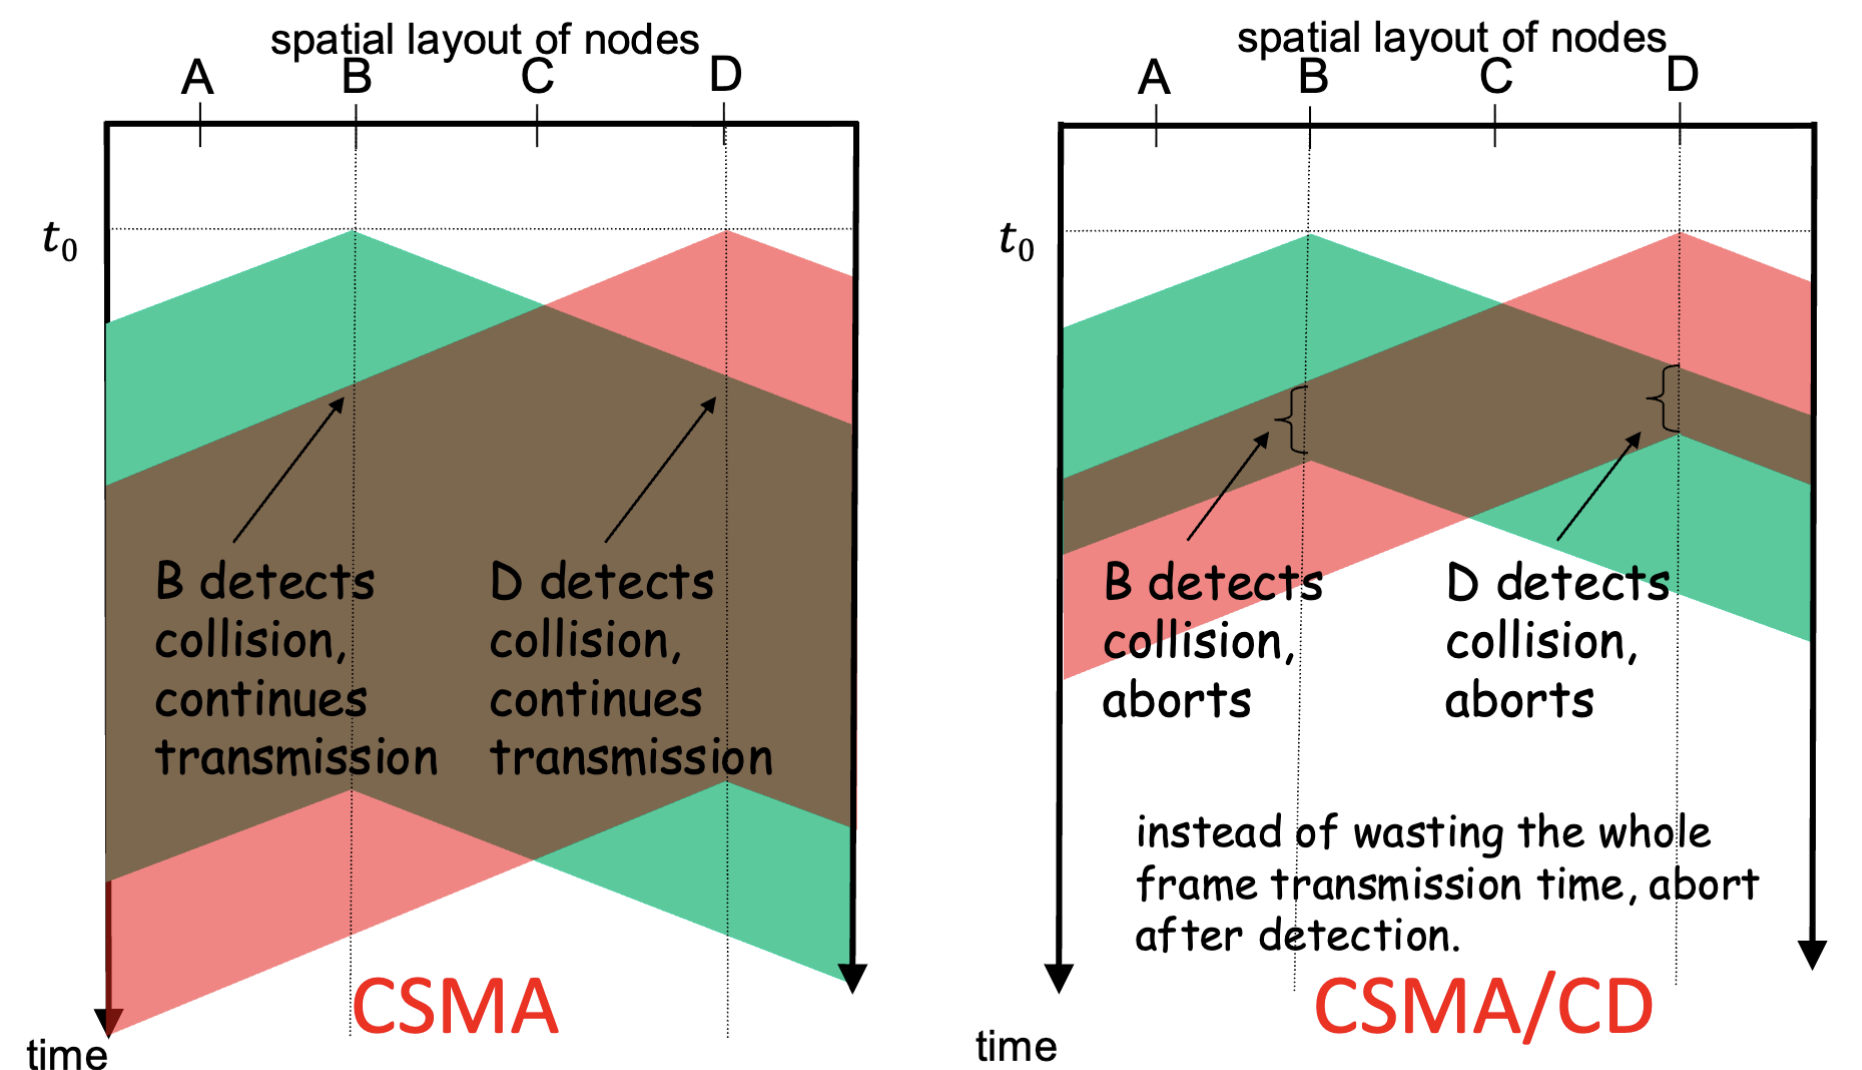
\includegraphics[width=0.75\linewidth]{link/csma.png}
\end{center}

\begin{center}
\resizebox{\columnwidth}{!}{%
  \begin{tabular}{lcccc}
    \hline
    \textbf{Protocol} & \textbf{Collision-Free} & \textbf{Efficiency} & \textbf{Fairness} & \textbf{Decentralized} \\
    \hline
    Slotted ALOHA
    & No
    & \(R\) one node; \(37\%\) many nodes
    & Perfectly fair
    & Yes \\

    Pure ALOHA
    & No
    & \(R\) one node; \(18\%\) many nodes
    & Perfectly fair
    & Yes \\

    CSMA / CSMA/CD
    & No
    & Yes
    & Yes
    & Yes \\
    \hline
  \end{tabular}%
}
\end{center}

Minimum Frame Size: $2\max\left(d_{\mathrm{prop}}\right) \leq d_{\mathrm{trans}}$ so that sending nodes can detect collision.
$d_{prop}$ d. prop. to diameter (maximum distance between any 2 nodes in the network)
$d_{trans}$ d. prop. frame size

\subsection{Taking Turns Protocols}
\textbf{Polling}
Master node polls each node in a round-robin fashion.
\begin{itemize}
\item Master informs node 1, it can transmit up to some $N_{max}$.
\item After node 1 transmits, master node tells node 2 it (node 2) can transmit up to $N_{max}$
\end{itemize}

\textbf{Token Passing}
Special frame, \textbf{token}, is passed from one node to
next. When node receives token, hold onto the token only if some frames to transmit. Otherwise, forward token
to next node. Cons: Token loss can disrupt the system, and a node failure can break the ring.

\begin{center}
\resizebox{\columnwidth}{!}{%
  \begin{tabular}{lccc}
    \hline
    \textbf{Protocol} & \textbf{Collision-Free} & \textbf{Efficiency} & \textbf{Decentralized} \\
    \hline
    Polling
    & Yes
    & Higher; polling overhead
    & No; master node as single point of failure \\

    Token Passing
    & Yes
    & Higher; token-passing overhead
    & Yes \\
    \hline
  \end{tabular}%
}

\vspace{2mm}
\textbf{Fairness:} Both are perfectly fair.
\end{center}

\subsection{Channel Partitioning Protocols}
\textbf{Time Division Multiple Access (TDMA)}
\begin{enumerate}
\item Channel access is divided into repeating rounds, or time frames.
\item Assign each node a fixed-length time slot for transmitting one data frame.
\item Unused nodes leave their slots idle (reduced efficiency).
\item E.g., for six nodes, nodes 1, 3, and 4 transmit while slots 2, 5, and 6 remain idle.
\end{enumerate}

\textbf{Frequency Division Multiple Access (FDMA)}
\begin{enumerate}
\item Channel spectrum is divided into frequency bands.
\item Each node is assigned a fixed frequency band.
\item Unused transmission time in frequency bands go idle.
\item E.g.: 6 nodes, 1, 3, 4 have frames, frequency bands 2, 5, 6 are idle.
\end{enumerate}

\begin{center}
\scriptsize
\resizebox{\columnwidth}{!}{%
  \begin{tabular}{lcccc}
    \hline
    \textbf{Protocol} & \textbf{Collision-Free} & \textbf{Efficiency} & \textbf{Decentralized} \\
    \hline
    TDMA & Yes & Inefficient; idle slots; max. throughput \(R/N\)
    & Yes \\

    FDMA & Yes & Inefficient; unused frequencies; max. throughput \(R/N\)
    & Yes \\
    \hline
  \end{tabular}%
}
\vspace{2mm}
\textbf{Fairness:} Both are perfectly fair.
\end{center}

\subsection{Error Detection}
\begin{center}
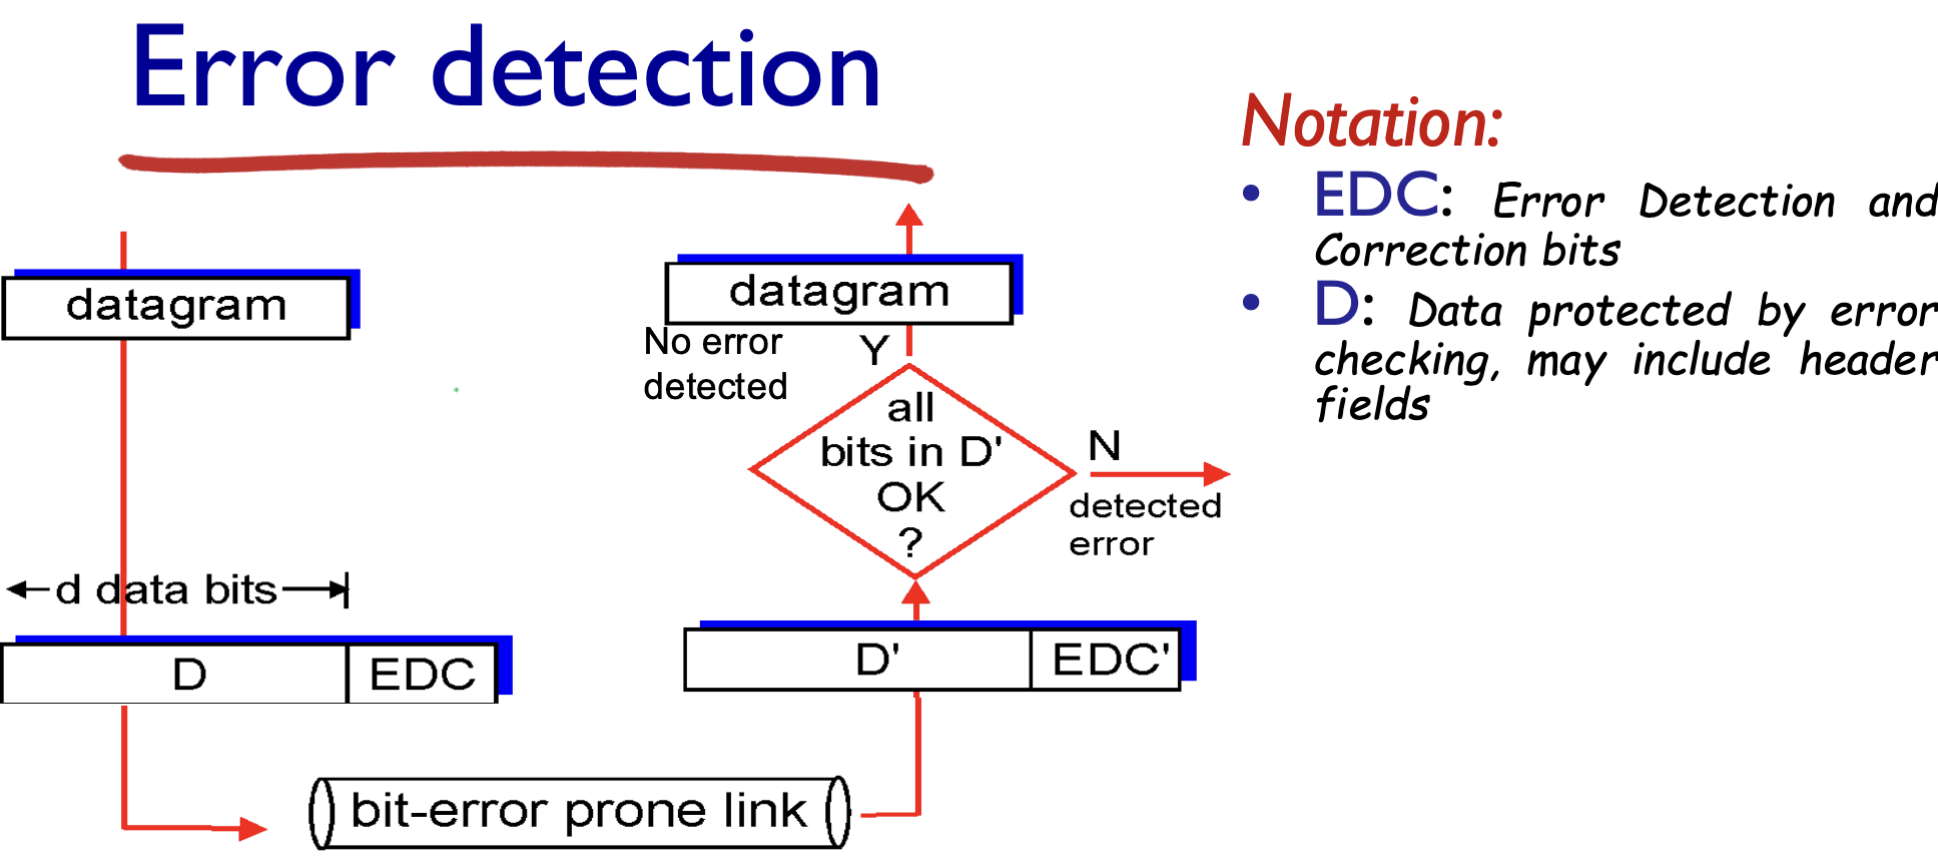
\includegraphics[width=0.75\linewidth]{link/error-d.png}
\end{center}

\textbf{Parity Checking}
Even Parity: sender simply includes one additional bit, chooses its value such that the total number of 1s in the
$d + 1$ bits is even.
\begin{center}
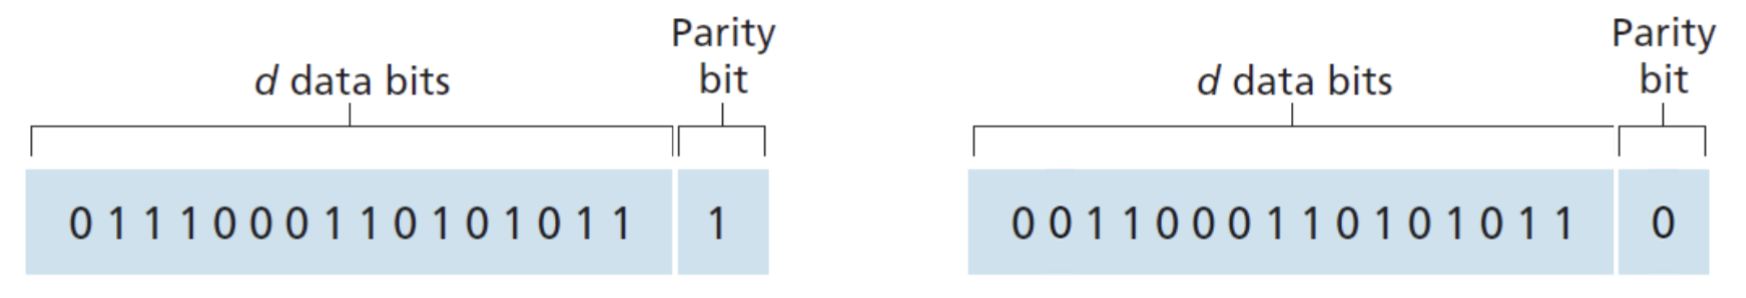
\includegraphics[width=0.75\linewidth]{link/parity.png}
\end{center}
Errors clustered in bursts - unable to detect even number of bit changes.
\textbf{Computing gradients}

2D Parity
\begin{center}
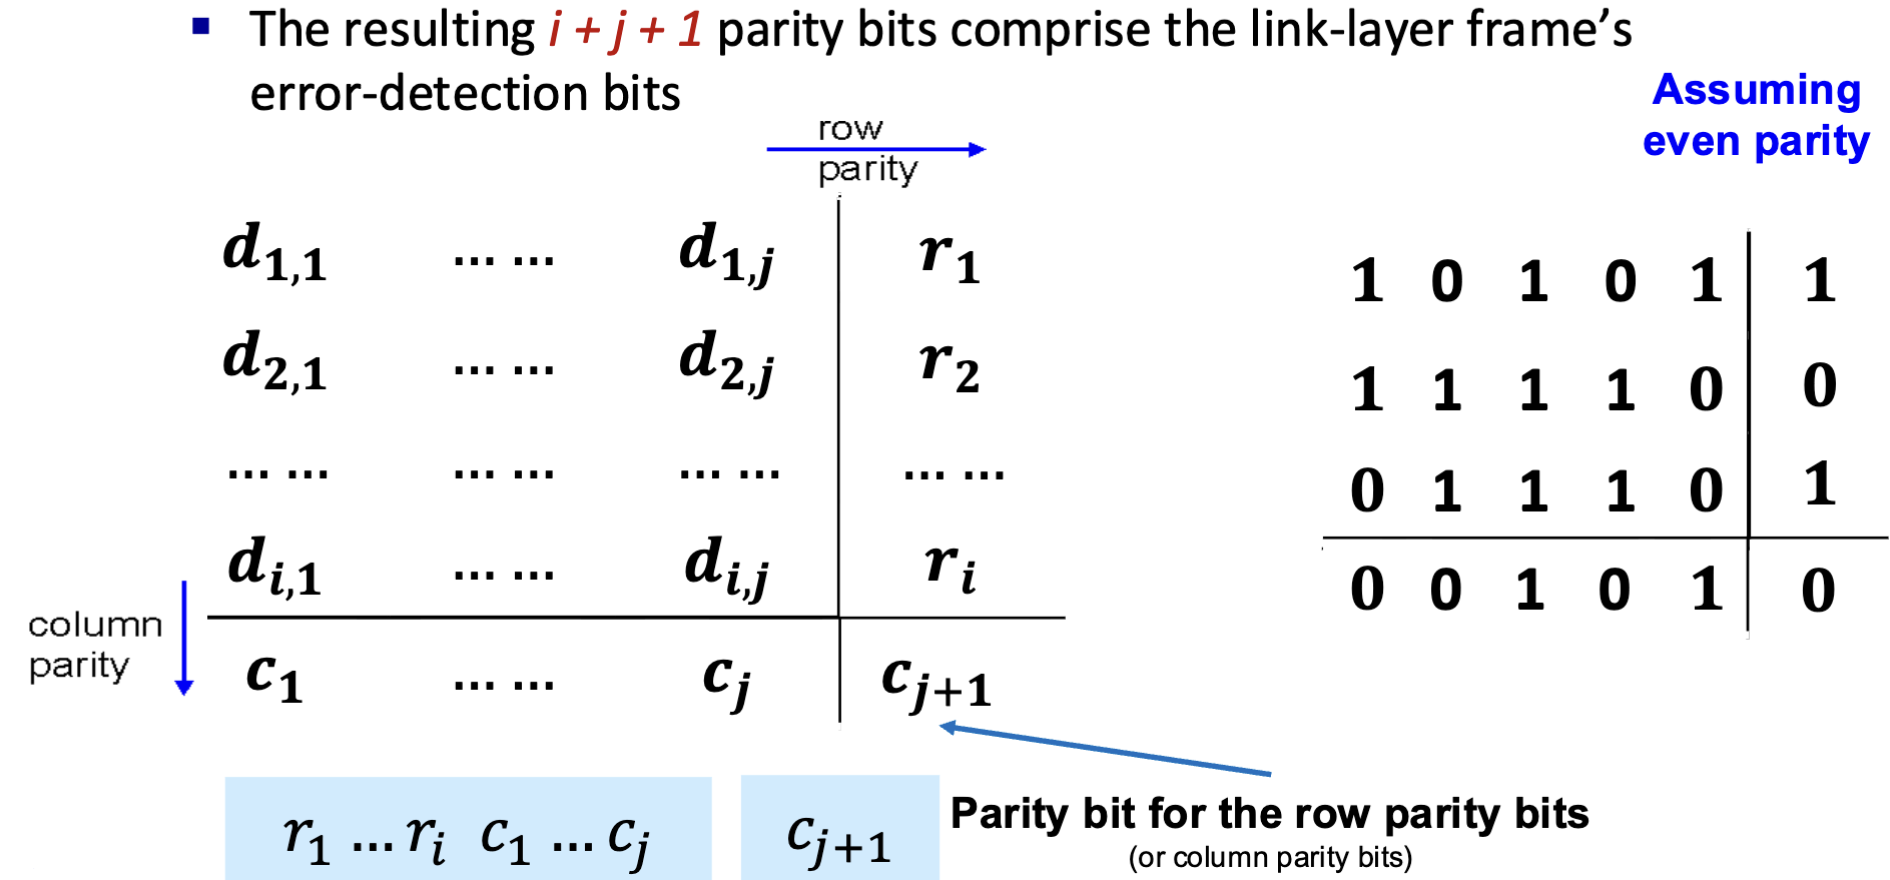
\includegraphics[width=0.75\linewidth]{link/2d.png}
\end{center}

\textbf{Cyclic Redundancy Check (CRC)}
\begin{center}
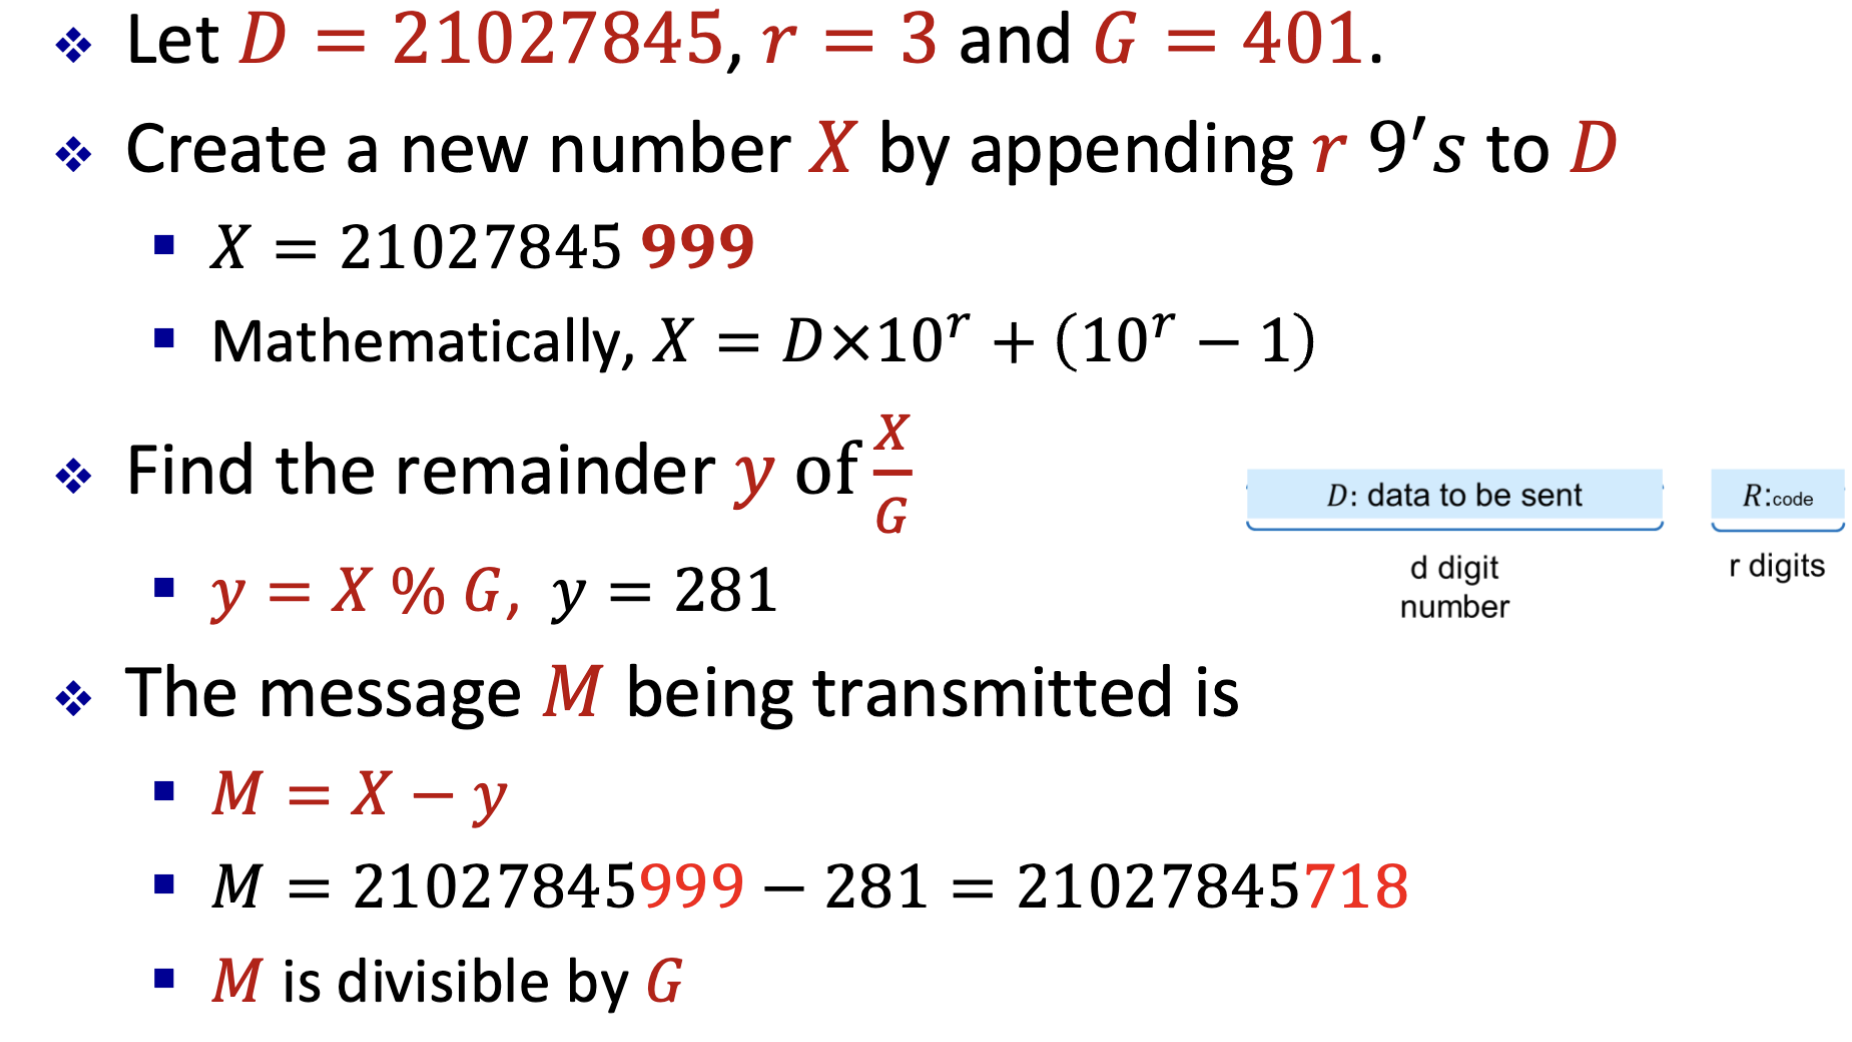
\includegraphics[width=0.48\linewidth]{link/crc.png}
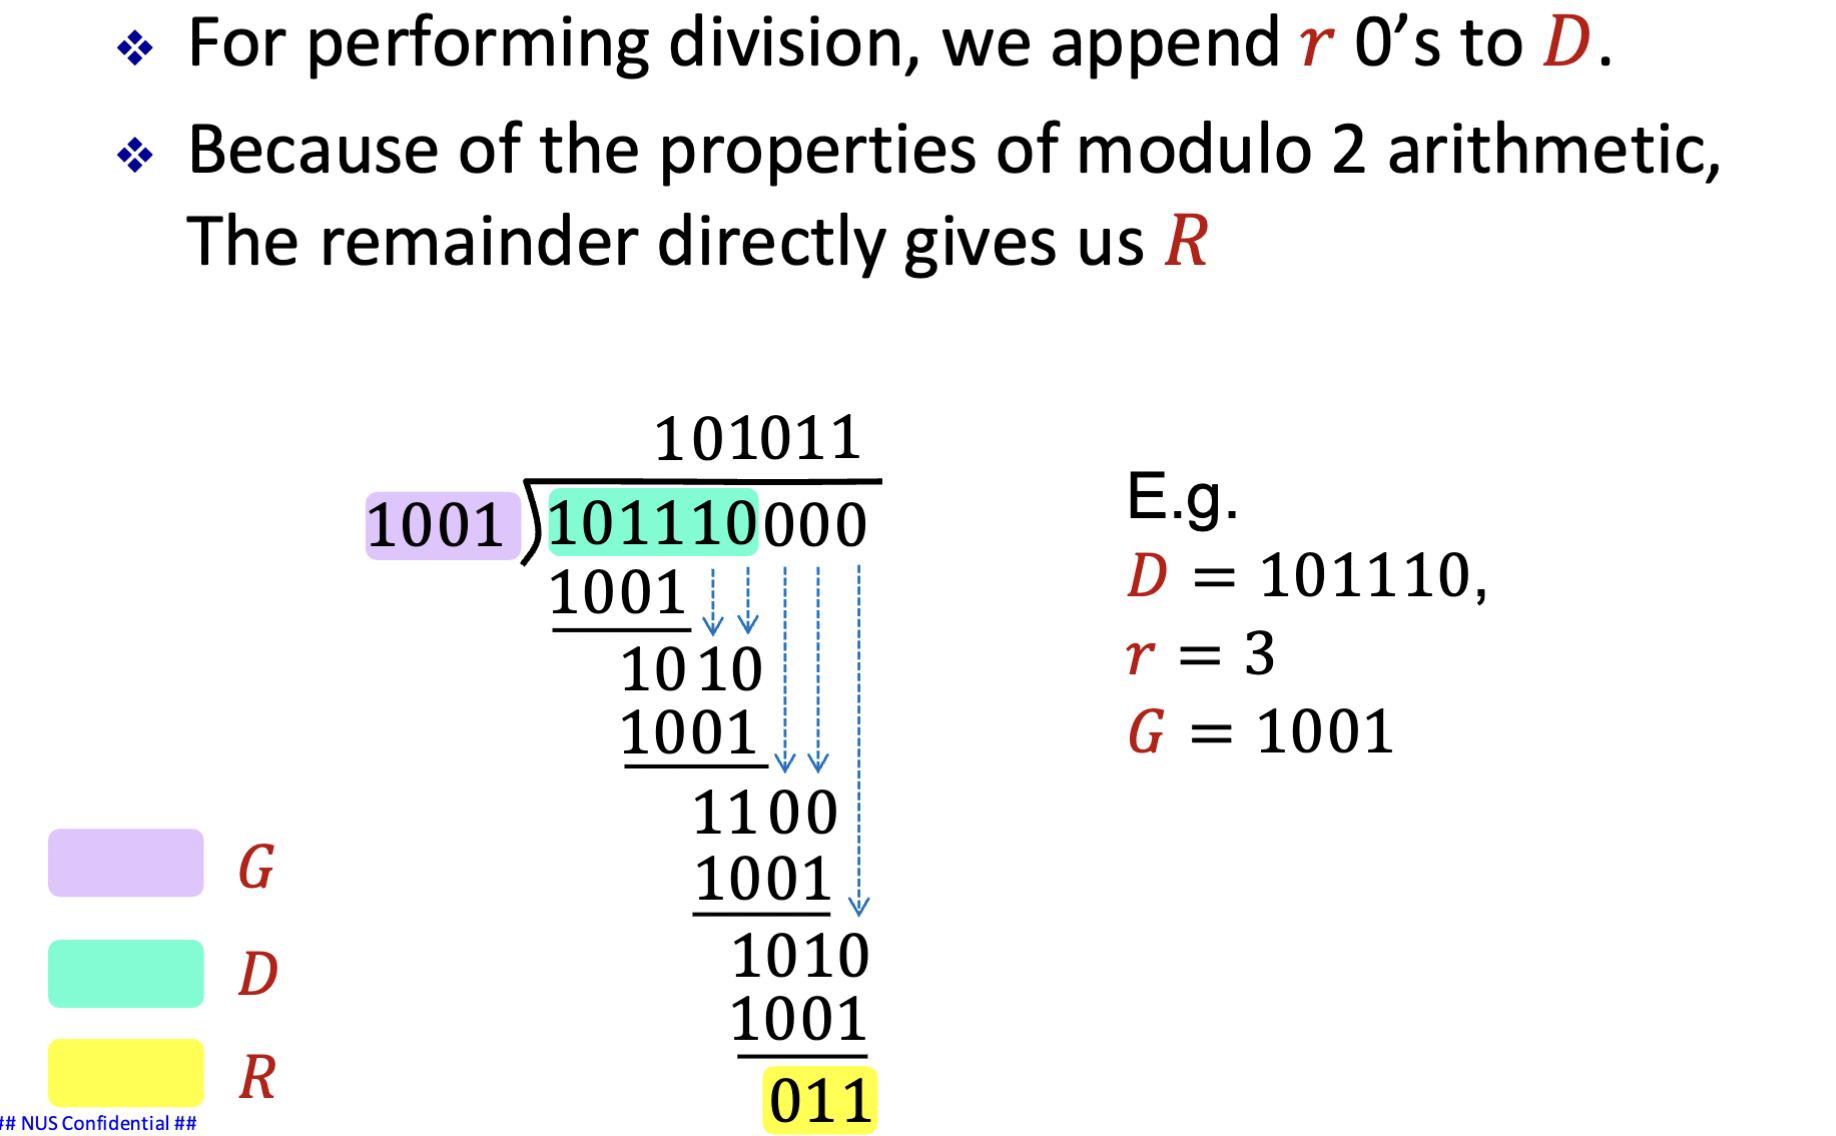
\includegraphics[width=0.48\linewidth]{link/crc-div.png}
\end{center}
Sender sends $(D, R)$. Receiver knows $G$, divide $(D, R)$ by $G$. Error when non-zero remainder.
Easy to implement on hardware, can detect all odd-number of single bit errors. CRC of $r$ bits can detect all burst errors of up to $r$ bits, and all burst errors of greater than $r$ bits with probability $1-0.5^r$

\subsection{Local Area Network (LAN)}
Computer network that interconnects computers within a geographical area such as office building or university campus.
\textbf{Ethernet}: considered the dominant LAN tech. Unreliable: receiving NIC doesn’t send ACK or NAK
to sending NIC. Uses CSMA/CD with exponential backoff.

\textbf{Ethernet Frame Structure}
\begin{center}
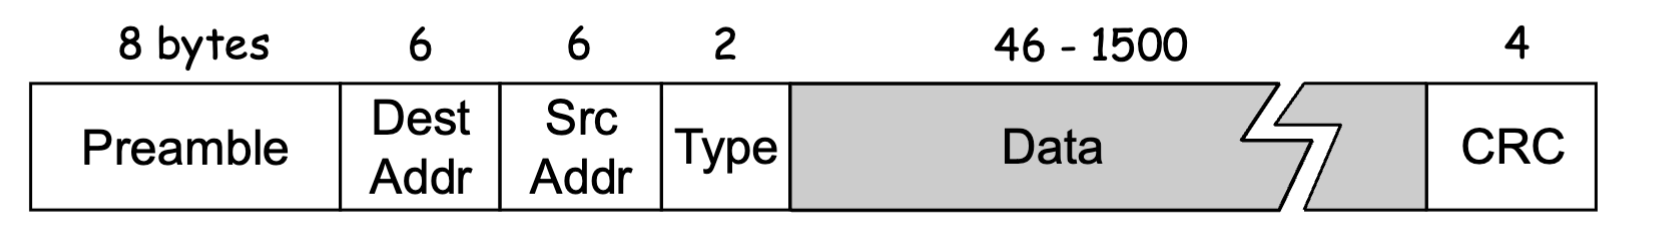
\includegraphics[width=0.75\linewidth]{link/ethernet-addr.png}
\end{center}
\textbf{Source \& Dest. MAC Addr}
If NIC receives a frame with matching destination MAC address, or with broadcast address, it passes data in the frame to network layer protocol. Otherwise, NIC discards frame.

\textbf{Data}
Max size: 1500 bytes (MTU). Min size: 46 bytes

\textbf{Type \& CRC}
Type identifies the enclosed upper-layer protocol (e.g. IP or ARP). CRC is
checked by the receiver; a corrupted frame is dropped. Ethernet itself has
no ACK/NAK, so any recovery is performed by a higher layer (e.g. TCP).

\textbf{Preamble}
7 bytes of pattern 10101010 (AAHex) + 1 byte of pattern 10101011 (ABHex) (i.e. `start of frame'). Used to synchronize receiver and sender clock rates. Used to tell receiver the "width" of a bit.
\par\vspace{2pt}\noindent\preamblediagram\par\vspace{2pt}

Interconnect the nodes to make a shared link:
\begin{enumerate}
\item \textbf{Bus} topology is a broadcast LAN. All transmitted frames received by all adapters connected to the bus (so all can collide). Slow, hard to troubleshoot.
\item \textbf{Star / hub} (physical layer). When a bit arrives from one interface, hub re-creates the bit, boosts energy strength, and transmits the bit onto all other interfaces. Modular, but slow esp for large networks.
\item \textbf{Star / switch} connect directly to nodes. Layer-2 device. Works on frames rather than individual bits. A bona-fide store-and-forward packet switch. No collisions
\end{enumerate}
\textbf{Hub vs. switch vs. router:} hub repeats bits to every port (one
collision domain); switch forwards frames using MAC addresses; router routes
IP datagrams between subnets and rebuilds the link-layer frame at each hop.

\textbf{Switch}
Examine incoming frame’s MAC address. Selectively forward frame to one-or-more outgoing links. Store and forward Ethernet frames. CSMA/CD to access link. Transparent (hosts are unaware of switches) and Plug-and-Play (self-learning).
A-to-A’ and B-to-B’ can transmit simultaneously, without collisions, but cannot send from A-to-A’ and B-to-A’ simultaneously.
Switch table tells which node is reachable by which interface. Format \texttt{< MAC address of host, interface to reach host, TTL >}. Update sender/location pair when frame is received.

\textbf{Forwarding rule:} first learn/update \texttt{< source MAC, incoming
interface >}. Look up destination MAC: known on a different port $\rightarrow$
forward only there; known on the incoming port $\rightarrow$ filter/drop;
unknown (or broadcast) $\rightarrow$ flood all ports except the incoming one.

\begin{center}
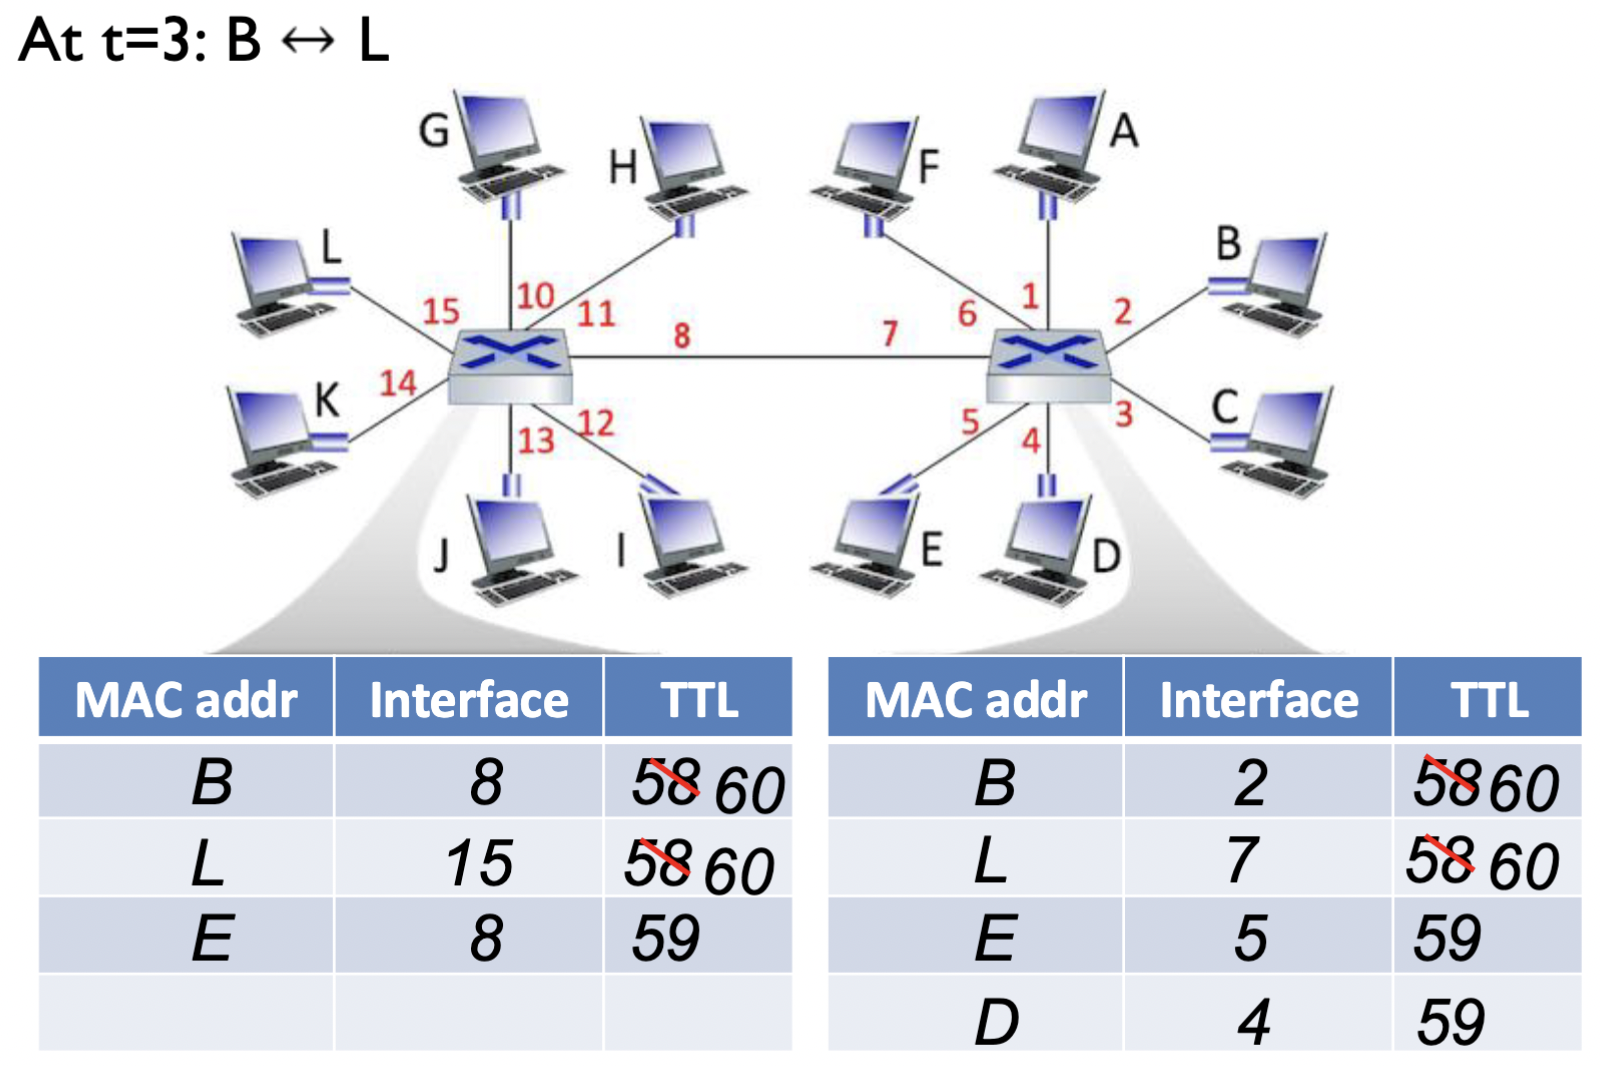
\includegraphics[width=0.75\linewidth]{link/switch-eg.png}
\end{center}

\subsection{MAC (Media Access Control) Address}
Every adapter (NIC) has a MAC address (aka physical or LAN address). Typically 48 bits, burned in NIC ROM. E.g. \texttt{5C-F9-DD-E8-E3-D2}.
Broadcast address: \texttt{FF-FF-FF-FF-FF-FF}.
First three bytes indicate vendor. Administered by IEEE.

\subsection{IP vs. MAC Address}
\begingroup
\renewcommand{\arraystretch}{1.05}
\begin{tabular}{@{}p{1.15cm}p{2.3cm}p{2.3cm}@{}}
\toprule
& \textbf{IP address} & \textbf{MAC address} \\
\midrule
\textbf{Layer / size} & Network (L3); IPv4 = 32 bits & Link (L2); normally 48 bits \\
\textbf{Purpose} & Route datagram to final destination & Deliver frame to next hop on one link \\
\textbf{Form} & Hierarchical: subnet prefix + host ID & Flat NIC/adapter identifier \\
\textbf{Lifetime} & Logical; can be assigned dynamically & Usually hardware-associated; normally stable \\
\bottomrule
\end{tabular}
\endgroup

\textbf{At a router:} remove incoming frame, route its IP datagram, then build a new frame. End-host IP src/dst normally stay the same; MAC src/dst change at every routed hop.

\subsection{Address Resolution Protocol (ARP)}
Query mechanism to learn a MAC address given an IPv4 address \emph{on the
same subnet}. Each IP node has an ARP table:
\texttt{< IP address; MAC address; TTL >}. ARP is plug-and-play; stale
mappings expire after the TTL.

\textbf{Within Same Subnet}
If A knows B’s MAC address from its ARP table, create a frame to B and send
it. Only B processes it; other NICs ignore it. On a cache miss, A broadcasts
an ARP query containing B's IP, with destination MAC
\texttt{FF-FF-FF-FF-FF-FF}. All local nodes receive it, but only B unicasts
its MAC reply; A caches the mapping, then sends the data frame. ARP broadcasts
do not cross routers.

\textbf{Sending to Different Subnets}
\begin{center}
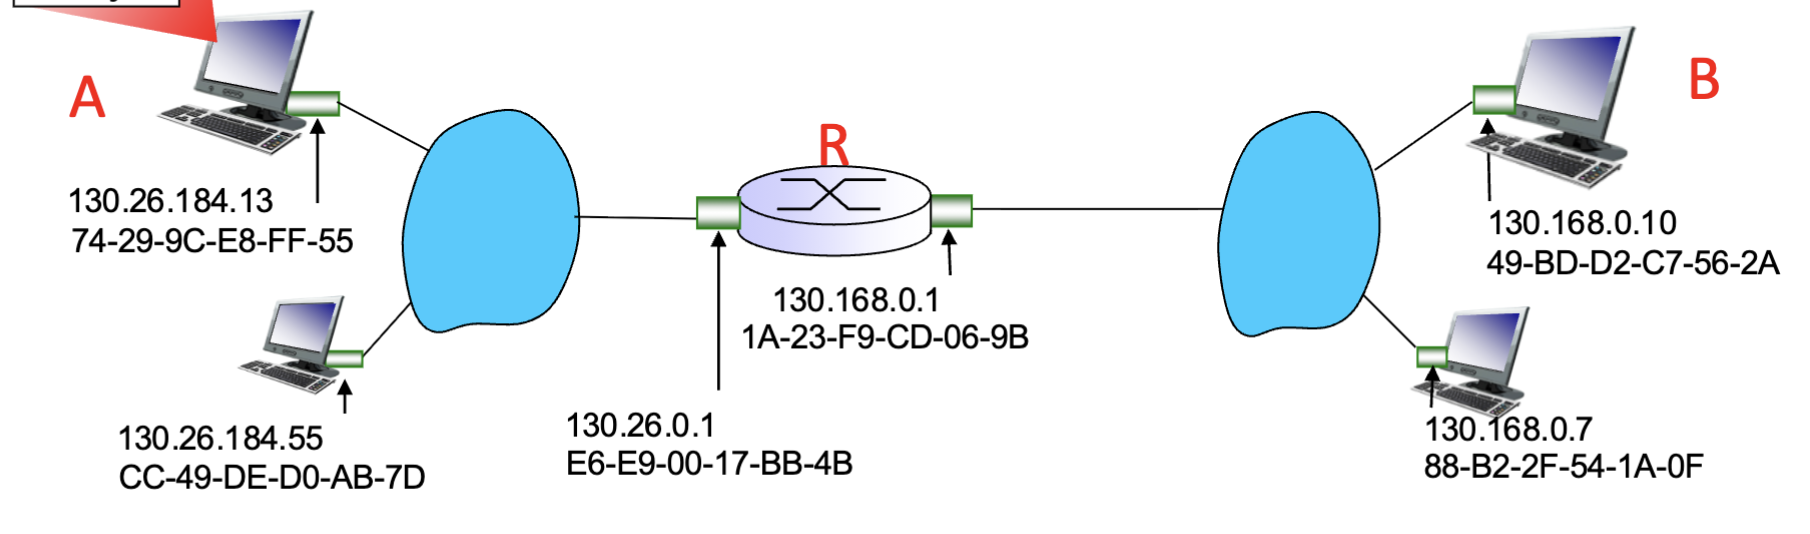
\includegraphics[width=0.75\linewidth]{link/guide.png}
\end{center}
\begin{enumerate}
\item A creates IP datagram with IP source A, final destination B.
\item A sees B is off-subnet, so it ARPs for its default gateway R's
  local-interface MAC (not B's remote MAC), if not already cached.
\item A sends a frame with MAC source A and MAC destination R, carrying
  the IP datagram A $\rightarrow$ B.
\item R removes the frame, routes using B's IP address, and resolves the
  MAC of the next hop on its outgoing link (B only if directly connected).
\item R builds a new frame: source MAC = its outgoing interface; destination
  MAC = that next hop. Every later router repeats this process.
\item Thus IP source/destination remain A/B end-to-end (apart from normal
  forwarding changes such as TTL), while source/destination MAC addresses
  change at every routed hop.
\end{enumerate}

\begin{center}
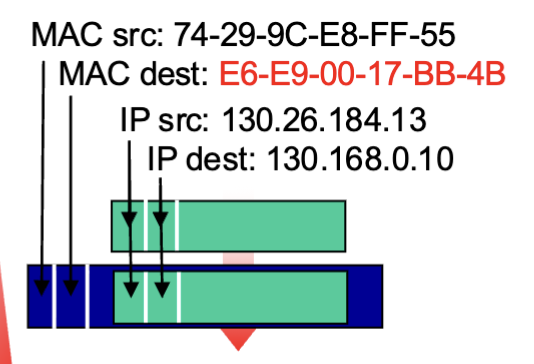
\includegraphics[width=0.32\linewidth]{link/datagram-a.png}
\hfill
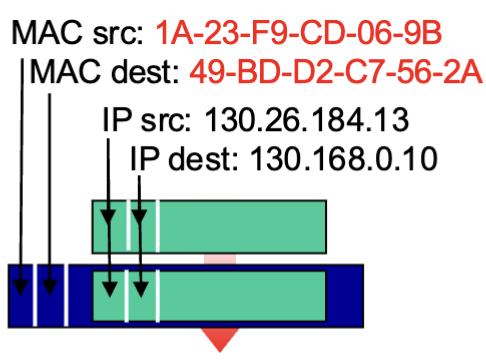
\includegraphics[width=0.32\linewidth]{link/datagram-r.png}
\hfill
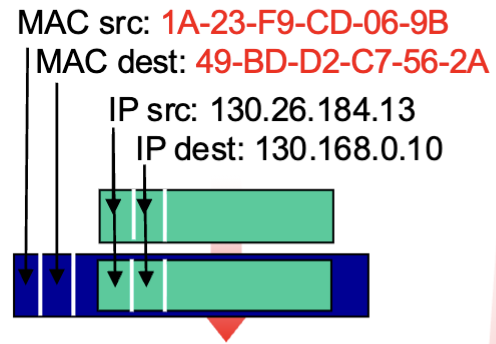
\includegraphics[width=0.32\linewidth]{link/datagram-b.png}
\end{center}

\subsection{Network Security}
\textit{Confidentiality} only sender, intended
receiver should `understand' message contents (no eavesdropping).
\textit{Message integrity} sender, receiver want to ensure message not altered (in transit, or afterwards) without detection (no modification)
\textit{Authentication} sender, receiver want to
confirm identity of each other (no impersonation or repudiation)
\textit{Nonrepudiation} Proving that a transaction happened between 2 entities

\subsection{Cryptography}
Allow a sender to disguise data so that an intruder can
gain no information from the intercepted data, and allow the receiver to recover the original data from the disguised data

\begin{center}
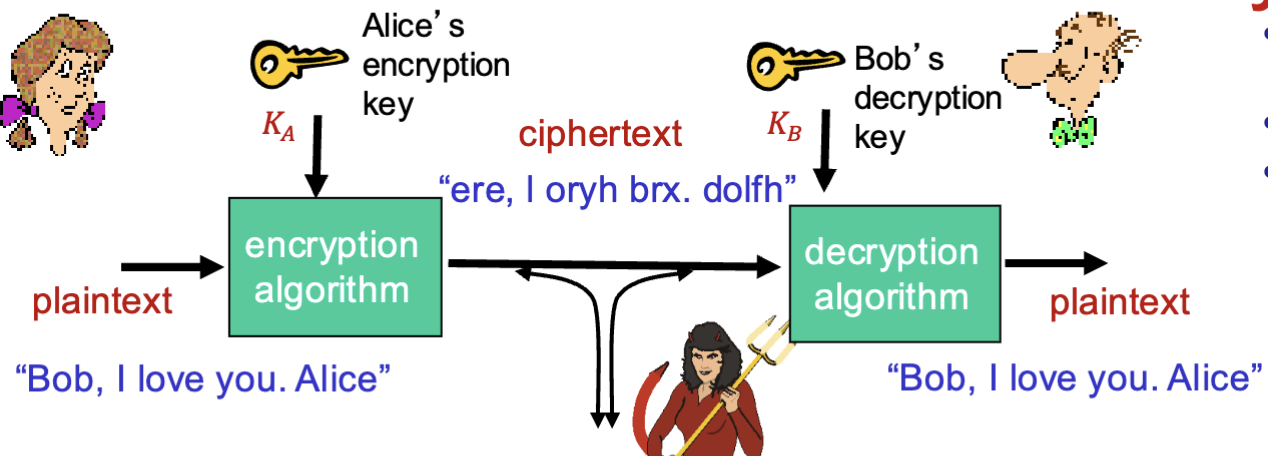
\includegraphics[width=0.75\linewidth]{security/notation.png}
\end{center}

\begin{itemize}
\item Symmetric Key Cryptography: $K_A = K_B$. E.g. Caesar cipher, monoalphabetic cipher -> can break with statistical analysis (known 2/3 letter combos)
\item Asymmetric Key Cryptography: $K_A \neq K_B$
\end{itemize}

\subsection{Symmetric Key Crypto}
Drawback: requires sender, receiver know to shared secret key. How to agree on this key?

\textit{Polyalphabetic encryption}
Use $n$ substitution ciphers.
\begin{center}
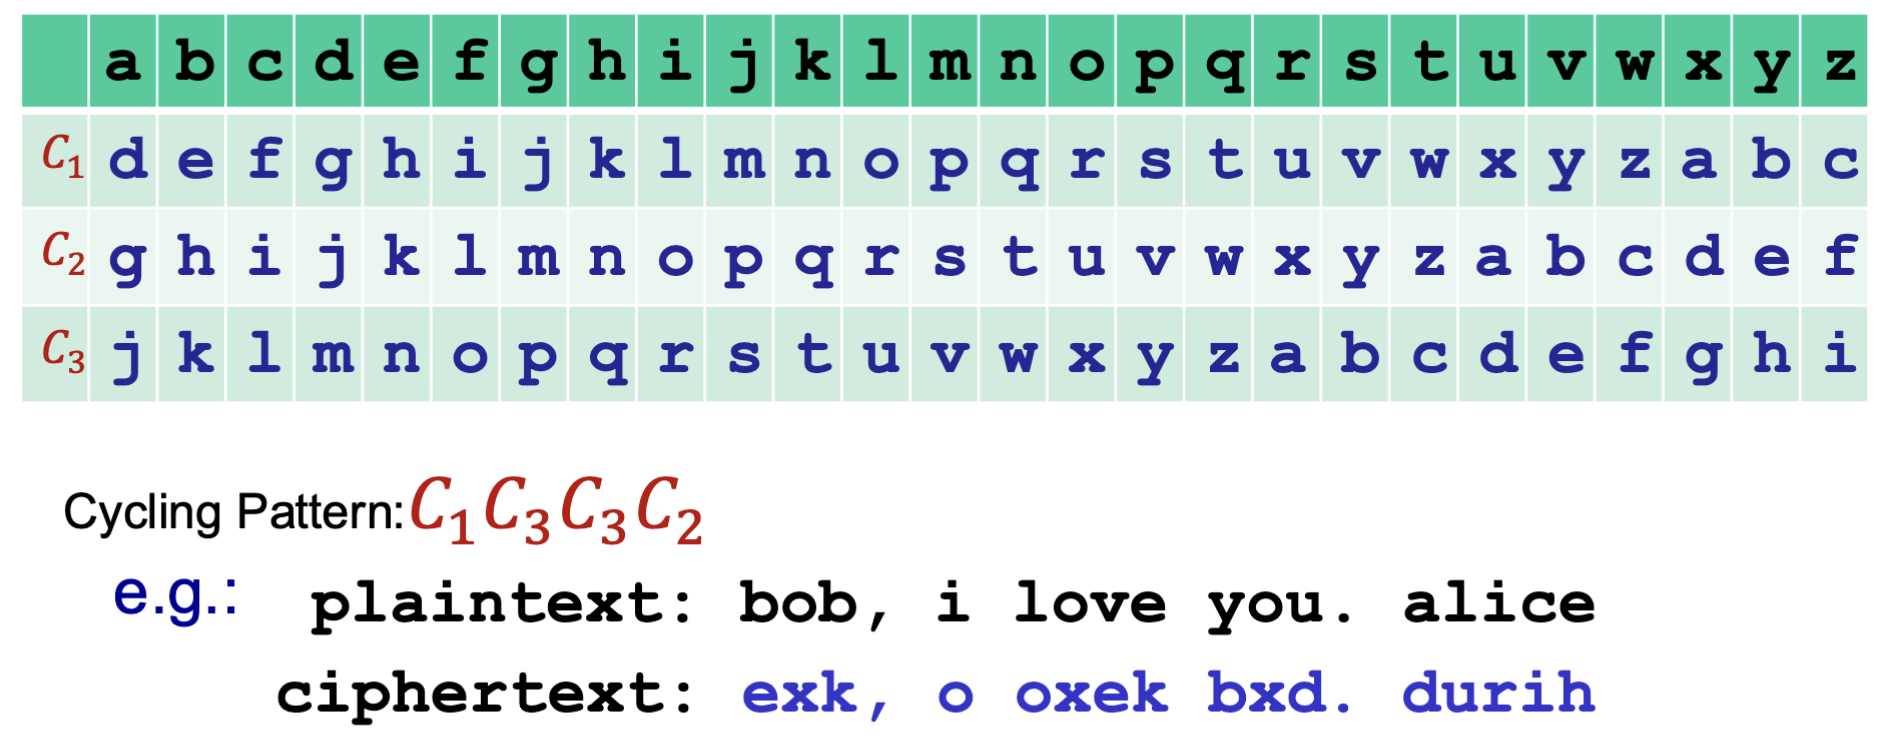
\includegraphics[width=0.75\linewidth]{security/poly.png}
\end{center}
Encryption key: $n$ substitution ciphers, and cycling pattern.

\textit{Block ciphers}
The message to be encrypted is processed in blocks of $K$ bits. Standards
\begin{enumerate}
\item DES: Data Encryption Standard (56-bit symmetric key, 64-bit block). 3DES more secure ver.
\item AES: Advanced Encryption Standard (128 bit blocks; 128, 192, or 256 bit keys).
\end{enumerate}

\textit{Public Key Cryptography}
Sender uses a public encryption key known to all. Receiver uses private decryption key known only to user.

\begin{center}
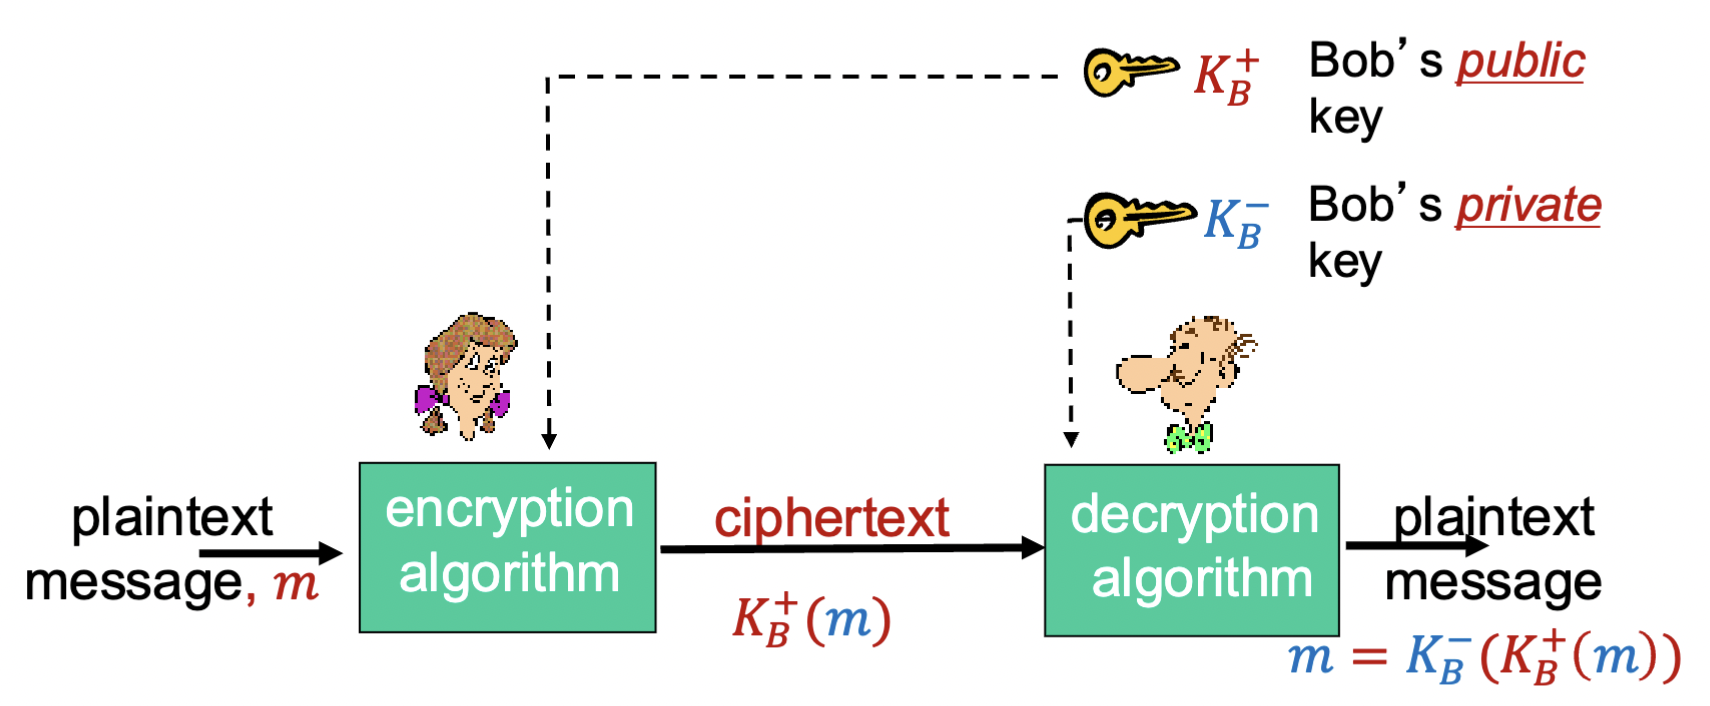
\includegraphics[width=0.75\linewidth]{security/public.png}
\end{center}

Given public key $K_B^+$, it should be impossible to compute private key $K_B^-$

\subsection*{RSA}
\textbf{Key generation}
\begin{enumerate}
\item Choose two large prime numbers \(p\) and \(q\).
\item Compute $n = pq, \qquad \varphi(n) = (p-1)(q-1)$.
\item Choose \(e\), where \(1 < e < \varphi(n)\), such that $\gcd(e,\varphi(n)) = 1$. \(e\) and \(\varphi(n)\) are relatively prime.
\item Choose \(d\) such that $ed \equiv 1 \pmod{\varphi(n)}$.
  Equivalently, \(ed-1\) is exactly divisible by \(\varphi(n)\).
\item $\text{Public key } K_B^+ = (n,e), \text{Private key } K_B^- = (n,d)$.
\end{enumerate}

\textbf{Encryption and decryption}
Given public key \((n,e)\) and private key \((n,d)\):

\begin{itemize}
\item To encrypt \(m<n\), compute $c \equiv m^e \pmod n$.
\item To decrypt ciphertext \(c\), compute $m \equiv c^d \pmod n$.
\end{itemize}

This is correct since $c^d \equiv (m^e)^d = m^{ed} \equiv m \pmod n$.

\textbf{Session keys}
To transfer a large file (M) from Alice to Bob
\begin{enumerate}
\item Alice generate a random session Key $K_S$
\item Encrypt and send key to Bob, using public key $K_B^+$
\item Bob extracts session key $K_B^-(K_B^+(K_S))$
\item Alice send M using symmetric key encryption using $K_S$
\end{enumerate}

\subsection{Message Integrity}
\textbf{Cryptographic Hash Function}
\textbf{Hash function:} A function $H(\cdot)$ that takes an input message $m$ and produces a fixed-size message digest, also called a \emph{fingerprint}. A hash function is many-to-one because messages of arbitrary length are mapped to outputs of fixed length. Faster than encryption.

\textbf{Cryptographic hash function:} Hash function where it is computationally infeasible to find two different messages $x \neq y$ such that $H(x) = H(y)$. Attacker cannot substitute one message for another while preserving its hash value.

e.g. \texttt{md5sum}. 128 bits. Small change in input results in large change in hash output. SHA.

\textbf{Message Authentication Code} Sender \& Receiver share authentication key $s$. Send Send $(m, H(m + s))$.

\textbf{Password Hashing} Passwords cannot be recovered only reset.
\begin{center}
\passwordhashdiagram
\end{center}

\textbf{Hashing: Timestamping}
\begin{itemize}
\item Produces a proof of work without revealing the work itself.
\item Submit hash of the work:
  \begin{itemize}
    \item The hash produces a timestamp representing the time of submission.
    \item The work can later be shown to be unmodified by recomputing
      and verifying its hash.
  \end{itemize}
\end{itemize}

\subsection{Digital Signatures}
Prove authentication. Sender (Bob) digitally signs document, establishing he is document owner/creator.

Signature must be
\begin{enumerate}
\item \textbf{Verifiable} Recipient (Alice) can check if the signature and the message was generated by Bob.
\item \textbf{Unforgeable} No one, other than Bob should be able to generate the signature and the message.
\end{enumerate}

Suppose Alice receives a message and signature pair: $\left(m, K_B^{-}(m)\right)$, where $K_B^{-}$ is Bob's private key.

Alice verifies signature using Bob's public key: $K_B^{+}\left(K_B^{-}(m)\right) = m$. If verification succeeds, Alice concludes that:
\begin{itemize}
\item Bob signed the message $m$;
\item the message was not signed by someone else;
\item Bob signed $m$, rather than a different message $m'$.
\end{itemize}
\textbf{Non-repudiation:} Alice can present $m$ and its signature $K_B^{-}(m)$ as evidence that Bob signed $m$. Since only Bob should possess his private key, Bob cannot credibly deny signing the message.

\textbf{Public Key Infrastructure (PKI)}
Public key distribution.
\textit{Certificate } digital document that contains identity and public key of owner, time window cert is valid, and signature of CA.
\textit{A CA} issues and signs digital certificates to websites/entities, maintains directory of public keys, and has its own public/private key pair. A CA binds public key to particular entity, E, while E registers its public key with CA, first by providing proof of identity. CA then creates cert binding E to a public key and signs it.
When Alice wants Bob’s public key, get Bob’s certificate (Bob or elsewhere) and apply CA’s public key to Bob’s certificate to get Bob’s public key

\subsection{Access and Availability}
Services must be accessible and available to users.

\textbf{Firewall} isolates organization’s internal net from larger Internet, allowing some packets to pass, blocking others. Prevents Denial of Service (DoS) attacks and illegal modification and/or access of data.

\textbf{Stateless Packet Filtering} Internal network connected to Internet via router firewall. Router filters packet-by-packet, decision to forward/drop packet based on source/dest IP address, TCP/UDP source and dest port numbers, ICMP message type, TCP SYN and ACK bits.

\begin{center}
\begingroup
\renewcommand{\arraystretch}{1.02}
\setlength{\tabcolsep}{2pt}
\scriptsize
\begin{tabular}{|>{\raggedright\arraybackslash}p{.38\linewidth}|>{\raggedright\arraybackslash}p{.48\linewidth}|}
  \hline
  \multicolumn{1}{|c|}{\textbf{Policy}} &
  \multicolumn{1}{c|}{\textbf{Drop rule}} \\
  \hline
  No external Web & Outbound TCP, destination port 80. \\
  \hline
  Only public Web server inbound & Inbound TCP SYN, except \texttt{130.207.244.203:80}. \\
  \hline
  Limit Web radios & Inbound UDP, except DNS and router broadcasts. \\
  \hline
  Prevent Smurf DoS & ICMP to directed-broadcast address. \\
  \hline
  Hide traceroute & Outbound ICMP ``TTL expired.'' \\
  \hline
\end{tabular}
\endgroup
\end{center}

ACL is a table of rules to apply to packets.
\begin{center}
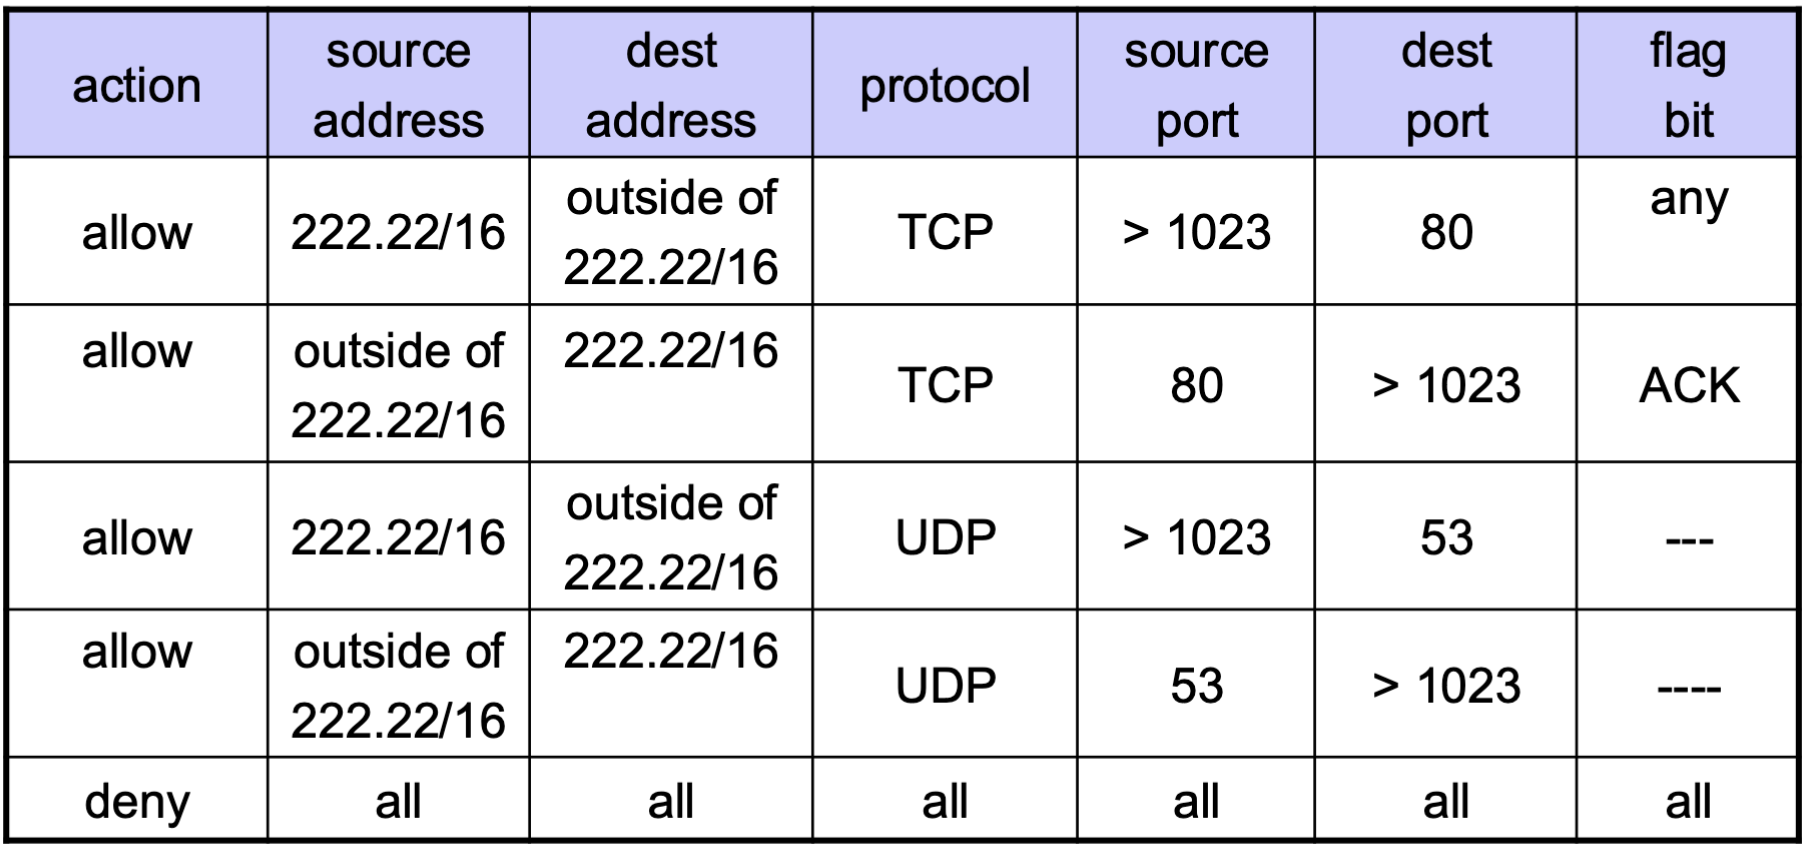
\includegraphics[width=0.75\linewidth]{security/acl.png}
\end{center}

Limitation: IP spoofing: router can’t know if data `really' comes from claimed source. Tradeoff: degree of communication with outside world limited.

\end{multicols}

\end{document}
